% interactcadsample.tex
% v1.03 - April 2017

\documentclass[]{interact}

\usepackage{epstopdf}% To incorporate .eps illustrations using PDFLaTeX, etc.
\usepackage{subfigure}% Support for small, `sub' figures and tables
%\usepackage[nolists,tablesfirst]{endfloat}% To `separate' figures and tables from text if required

\usepackage{natbib}% Citation support using natbib.sty
\bibpunct[, ]{(}{)}{;}{a}{}{,}% Citation support using natbib.sty
\renewcommand\bibfont{\fontsize{10}{12}\selectfont}% Bibliography support using natbib.sty

\theoremstyle{plain}% Theorem-like structures provided by amsthm.sty
\newtheorem{theorem}{Theorem}[section]
\newtheorem{lemma}[theorem]{Lemma}
\newtheorem{corollary}[theorem]{Corollary}
\newtheorem{proposition}[theorem]{Proposition}

\theoremstyle{definition}
\newtheorem{definition}[theorem]{Definition}
\newtheorem{example}[theorem]{Example}

\theoremstyle{remark}
\newtheorem{remark}{Remark}
\newtheorem{notation}{Notation}

% see https://stackoverflow.com/a/47122900


\usepackage{hyperref}
\usepackage[utf8]{inputenc}
\usepackage{dcolumn}
\def\tightlist{}


\begin{document}

\articletype{}

\title{Working from home and digital divides: resilience during the
pandemic}


\author{\name{Hannah Budnitz$^{a}$, Emmanouil Tranos$^{b, c, \dagger}$}
\affil{$^{a}$Transport Studies Unit, University of Oxford,
UK; $^{b}$School of Geographic Sciences, University of Bristol,
UK; $^{c}$The Alan Turing Institute, UK; $^{\dagger}$Corresponding
author}
}

\thanks{CONTACT Hannah
Budnitz. Email: \href{mailto:hannah.budnitz@ouce.ox.ac.uk}{\nolinkurl{hannah.budnitz@ouce.ox.ac.uk}}, Emmanouil
Tranos. Email: \href{mailto:e.tranos@bristol.ac.uk}{\nolinkurl{e.tranos@bristol.ac.uk}}}

\maketitle

\begin{abstract}
This paper offers a new perspective on telecommuting from the viewpoint
of the complex web of digital divides. Using the UK as a case study,
this paper studies how the quality and reliability of internet services,
as reflected in \emph{experienced} internet upload speeds during the
spring 2020 lockdown, may reinforce or redress the spatial and social
dimensions of digital divisions. Fast, reliable internet connections are
necessary for the population to be able to work from home. Although not
every place hosts individuals in occupations which allow for
telecommuting nor with the necessary skills to effectively use the
internet to telecommute, good internet connectivity is also essential to
local economic resilience in a period like the current pandemic.
Employing data on individual broadband speed tests and state-of-the-art
time-series clustering methods, we create clusters of UK local
authorities with similar temporal signatures of experienced upload
speeds. We then associate these clusters of local authorities with their
socioeconomic and geographic characteristics to explore how they overlap
with or diverge from the existing economic and digital geography of the
UK. Our analysis enables us to better understand how the spatial and
social distribution of both occupations and online accessibility
intersect to enable or hinder the practice of telecommuting at a time of
extreme demand.
\end{abstract}

\begin{keywords}
covid; internet; working from home; broadband speed; time-series
clusters
\end{keywords}

\hypertarget{sec:1}{%
\section{Introduction}\label{sec:1}}

During the pandemic, working from home using digital technologies,
whether partially or exclusively, was transformed from a niche means of
accessing work, albeit one that had been on a slow, upward trend, to a
widespread way of life in many countries. The ability to work from home
or telecommute meant millions retained their jobs and, to a varying
extent, maintained productivity during periods of strict lockdowns
around the world. However, this ability has not been evenly distributed
socially or spatially, creating new intersections of economic and
digital divisions. On one side are those who can work from home,
supported by digital technologies, and have thus been able to enjoy both
economic resilience and greater personal safety. On the other side,
previously employed individuals have been forced to accept furlough or
redundancy packages unless they are part of the cadre of essential
workers, who are potentially at high risk of infection. Whilst the basis
for this pandemic-generated divide has been viewed as mainly
occupational, here we consider whether it is also technological and
geographical.

The capability to work from home has previously been studied from the
perspective of whether work tasks in a given occupation both can be and
are allowed to be performed using digital technologies independently of
location or co-location with colleagues, including supervisors
\citep{allen2015effective, singh2013modeling}. However, successful
telecommuting also requires that the quality and reliability of digital
services, particularly home internet connection speeds, enable the
completion of work tasks with a minimum of delay or interruption. High
levels of demand are one of the main causes of reduced reliability and
slower connection speeds, as network bandwidth becomes congested. Yet
prior to the pandemic, the performance of broadband services with
respect to telecommuters was never tested at scale, as working from home
and connecting to colleagues and workplace resources via the internet
was the purview of a small minority of workers. Instead, leisure use in
the evening, when video streaming services are at their peak, has been
used to benchmark broadband performance and service delivery by
different Internet Service Providers (ISPs) \citep{ofcom2017}.

The shift towards telecommuting during various stages of lockdown around
the world has been drastic and there are speculations that post-Covid,
the tendency to work from home will be much higher, raising questions
around whether internet services can accommodate the increased demand.
For example, \(47\)\% of people in employment in the UK worked solely
from home in April \(2020\), whilst the same figure only reached \(5\)\%
the year before \citep{ons2020, ons2020lm2019}. Similar figures have
been reported for other countries \citep{felstead2020homeworking}.
Approximately \(37\)\% of the European workforce worked from home in
April \(2020\) with countries like Finland reaching \(60\)\%
\citep{eurofound2020}. In the US, almost half of the working population
worked from home during the same period because of the pandemic
\citep{brynjolfsson2020covid}, and a recent estimate indicated that
\(37\)\% of all jobs in the US can be permanently performed entirely
from home \citep{NBERw26948}. None of these changes could have happened
in the absence of reliable information and communication technology
(ICT) infrastructure -- both in terms of software and hardware. But
while software innovations are easily diffused across space and
society\footnote{See for example the huge success of videoconferencing
  apps such as Zoom \citep{marks2020zoom}.}, the same does not apply for
ICT hardware infrastructure such as internet broadband connectivity.

Using the UK as a case study, this paper aims to understand how the
quality and reliability of internet service, as reflected in
\emph{experienced} internet speeds during the spring 2020 lockdown, may
reinforce or redress the spatial and social dimensions of digital
divisions. We employ volunteered geographic data on individual broadband
speed tests and state-of-the-art time-series clustering methods to
create clusters of UK local authorities with similar temporal signatures
of experienced internet speeds. We then associate these clusters of
local authorities with their socioeconomic and geographic
characteristics to explore how they overlap with or diverge from the
existing economic and digital geography of the UK. As the quality of
internet infrastructure and services, as well as the concentration of
different occupations are spatially dependent and clustered in space,
our approach offers a framework for understanding the impact of and
interactions between digital divisions geographically and
socioeconomically. Our analysis enables us to better understand how the
spatial and social distribution of occupation and online accessibility
intersect to enable or hinder the practice of telecommuting at a time of
extreme demand. We also consider what lessons can be learned from this
time for a future where telecommuting is likely to remain a more common
means of accessing work, at least in comparison to the pre-Covid era.

By asking how resilient broadband speeds, and particularly upload
speeds, are as experienced in different parts of the UK during a time of
extreme demand, we interrogate which places benefit from the greater
economic resilience digital technologies can offer. The structure of
this paper is as follows. First we review the literature on
telecommuting and digital divides to better understand their structural
and spatial development pre-pandemic, and thus their importance to the
economic resilience of different places. We then describe our data and
methodology. Our results section first offers a classification of how
internet services vary across clusters of UK local authorities and then
assesses whether these clusters replicate or repudiate other
socio-economic and geographic patterns of economic resilience. We
conclude with a discussion of the insights we have gained from our new
perspective on digital divisions.

\hypertarget{sec:2}{%
\section{Literature review}\label{sec:2}}

\hypertarget{sec:2.1}{%
\subsection{From telecommuting to \#WFH}\label{sec:2.1}}

In this analysis, the terms `telecommuting' and `working from
home\footnote{See also the popular social media hashtag \#WFM}' are used
interchangeably, as most remote labour during the Covid-19 crisis was
carried out in the homes of individual employees rather than any other
location \citep{eurofound2020}. However, previous research has explored
how telecommuting can occur in other places, including satellite offices
or on public transport \citep{felstead2012rapid, siha2006telecommuting}.
Previous research has also used a variety of definitions to measure the
level of telecommuting within different workforces, distinguishing
between those directly employed, indirectly employed, self-employed,
full-time or part-time, and those who use digital technologies to work
remotely full-days or part-days
\citep{allen2015effective, bailey2002review, haddad2009examination}. No
matter the definition, the option and capability to telecommute or work
from home has never been equally distributed spatially or
socio-economically any more than different industries and employment
opportunities have. Studies from the United States, the Netherlands, and
the UK found that telecommuters are most likely to hold professional,
managerial, and technical occupations where the workforce is better
educated and wealthier, and that there is suppressed demand among women
and part-time workers
\citep{headicar2016move, peters2004employees, singh2013modeling}.

Opportunities for working from home during the current pandemic have
likewise not been equally spread across the workforce.
\citet{NBERw26948} indicated that in the US, managers, educators, those
working in computer-related occupations, finance, and law can easily
work from home, and that occupations with opportunities to telecommute
are associated with higher earnings. This is not the case for the
workforce occupied in more spatially fixed occupations, from farming,
construction and manufacturing to hospitality and care services. In the
US, these occupations tend to be lower-income, non-white, without a
university degree, live in rental accommodation and lack health
insurance \citep{NBERw27085}. Similar trends can be observed for other
countries. For example, \(75\)\% of workers with tertiary education
worked from home in Europe during spring \(2020\), whilst only \(34\)\%
of workers with secondary education and \(14\)\% of those primary
education did so \citep{eurofound2020}.

\hypertarget{sec:2.2}{%
\subsection{Digital divides and economic resilience}\label{sec:2.2}}

The literature describes first level digital divides in terms of the
availability and quality of internet connectivity, such as that manifest
in different geographies in the UK
\citep{riddlesden2014broadband, philip2017digital}. Second level digital
divides consider the presence or lack of the necessary skills to
effectively utilise digital technologies and the internet
\citep{blank2014dimensions, van2011internet}. The third level focuses on
the heterogenous returns of internet usage among different socioeconomic
groups and, consequently, how digital technologies can assist in
bridging or further enhancing existing socioeconomic divides.
\citep{stern2009levels, van2014digital, van2015third}. The potential for
these different levels of digital divide to interact is growing in
parallel with the digitisation of various sectors of the economy and
society. For example, \citet{li2020challenges} highlights how the
intersection of new demands upon ICT infrastructure and a paucity of end
users means that some areas are being left behind in the roll-out of
smart applications and services. They argue that this could create a
geospatial `smart divide', with areas unable to capitalise on the
opportunities offered by such applications and services. Likewise, the
capability to telecommute is related to all three levels of digital
divides, but more importantly leads to differentiated outcomes regarding
the economic resilience of people and places to overcome a systemic
shock such as the current pandemic.

Our understanding of telecommuting as a product of enabled occupations
can be described as a manifestation of the third level digital divide,
as those who are able to use digital technologies to work from home
benefit from a high rate of return on their use of the internet in terms
of autonomy, flexibility, and time saved from commuting
\citep{peters2004employees, siha2006telecommuting, singh2013modeling}.
In some aspects, these returns may have increased during the Covid-19
crisis, when those with the capability to telecommute also have the
ability to maintain their employment whilst protecting their health.
However, the success of these arrangements has been dependent upon the
first level digital divide, which is associated with geospatial access
to and quality of internet connectivity. \citet{SALEMINK2017360}
provides a systematic review of the pre-pandemic, first level digital
divide in infrastructure quality between urban and rural areas in
various advanced economies. Rural areas, predictably, fare worse. This
finding broadly applies in the UK, where studies that also analysed
broadband speed checks concluded that average speeds are lower in rural
areas, something that has not been improved by policy measures to
increase competition
\citep{riddlesden2014broadband, nardotto2015unbundling}. In contrast,
\citet{riddlesden2014broadband} found that levels of deprivation did not
correlate with first level digital divides, perhaps because many
deprived areas benefit from spillover effects of quality installed
infrastructure nearby.

However, as \citet{blank2018local} highlight, variation in individual
internet availability and uptake is a product of more complex geospatial
and demographic characteristics than simple rurality, urbanisation or
levels of deprivation. Dense urban areas were shown to suffer more from
slowdown during peak hours, although these services were more likely to
be improved by increased competition between providers, such as between
new entrants and Virgin Media cable connections
\citep{riddlesden2014broadband, nardotto2015unbundling}. The latter were
historically available to only \(45\)\% of premises in the UK
\citep{ofcom2016}, where the more lucrative and competitive market
originally attracted the cable TV provider. Whether the geospatial
variation in infrastructure quality and reliability affects the spatial
footprint of telecommuting has not previously been investigated, in part
because telecommuting has not previously been a cause of concentrated
demand and pressure on internet services.

Other intersections between digital divides have been subject to study.
There are indications that those who purchase high speed connections
consume more data of all sorts and use their connections for a greater
variety of purposes \citep{hauge2011consumer}. There is also a
correlation between access to internet services and a reduction in
household transport spend \citep{bris2017ict}. These studies suggest
that better internet services enable households to make savings and
efficiencies, an example of the first level digital divide reinforcing
the third level. Such digital intersections and efficiencies have also
changed transportation, connectivity and the structure of cities during
the pandemic. We now have enough data to confirm the drastic alteration
observed in the space-time geography of cities around the world in the
last year \citep[e.g.][]{google2020, shibayama2021impact}. Yet, although
there is a broad agreement that these changes during the pandemic have
played a pivotal role in stopping the spread of the virus
\citep{jia2020population, yang2020taking, mu2020interplay}, the extent
to which the increased levels of working from home, the consequent
decrease in commuting flows, and the altered structure of cities will
remain post-pandemic is the subject of considerable debate in the
literature.

Meanwhile, multi-layered digital divides may also intersect with
material divides and the economic geography of the UK. The regional
economic resilience literature underlines the differentiated capacity of
cities and regions to escape or recover from economic crises
\citep{martin2012regional, kitsos2018economic}. As different places have
different industrial and occupational profiles, these affect their
aggregated potential capacity for telecommuting. Such profiles are
associated with longstanding inequalities in the UK and their spatial
representation as a North-South divide \citep{martin_north_south}.
Various studies have illustrated severe inequalities between the north
and the south regions of England in terms of skills and human capital,
unemployment, productivity and prosperity
\citep{lee2014grim, mccann2020perceptions, dorling2018peak}. Some
scholars have even argued that the UK suffers from some of the highest
levels of interregional inequalities in the global north
\citep{gal2018reducing, mccann2016uk}. All three levels of digital
divides are associated with or shaped by the geography of the UK. Yet
this is the first time that the intersection of digital and material
divides is relevant to understanding the economic resilience of places
and large swathes of the population, as digital technologies became an
essential tool of productivity during the Covid-19 pandemic.

The extreme demand during the pandemic thus provides a new opportunity
to understand how internet infrastructure quality, and reliability
affects telecommuting, particularly in light of the high volumes of
bandwidth-intensive video conferencing required in order to avoid the
face-to-face contact that could increase the spread of infection. We
seek to answer how internet service resilience could contribute to or
reduce economic resilience when the latter is dependent upon the
capability to work from home. We also aim to improve our understanding
of the impact of first level digital divisions on telecommuting, in
terms of both geospatial and temporal quality of service, and whether
this results in more fundamental third level digital divisions between
local geographies than has previously been perceived.

\hypertarget{sec:3}{%
\section{Methods and data}\label{sec:3}}

\hypertarget{sec:3.1}{%
\subsection{Time-Series clustering}\label{sec:3.1}}

Our chosen methodological framework is cluster analysis, which can be
defined within machine learning approaches as an unsupervised learning
task, partitioning unlabelled observations into homogeneous groups known
as clusters \citep{montero2014tsclust}. The key idea is that
observations within clusters tend to be more similar than observations
between clusters. Clustering is particularly useful for exploratory
studies as it identifies structures within the data
\citep{aghabozorgi2015time}. Cluster analysis is a widely used in
geography \citep{gordon1977classification, everitt1974cluster}, for
example to solve \emph{regionalisation} problems
\citep{niesterowicz2016}. Clustering methods are also the basis of
\emph{geodemographics}, a research domain which aims to create small
area indicators or typologies of neighbourhoods based on diverse
variables \citep{SINGLETON2009289, harris2005geodemographics}. These
studies usually employ cross-sectional data, and most clustering
problems in geography deal with observations that are fixed in time.
However, for this paper we are interested in internet speeds, which vary
over time. Therefore, we create clusters of local authorities in the UK
with similar temporal signatures of experienced internet speeds.

To do so, we employ time-series clustering methods, which have been
developed to deal with clustering problems linked to, for instance,
stock or other financial data, economic, governmental or medical data as
well as machine monitoring
\citep{aggarwal2013time, aggarwal2001surprising, hyndman2015large, WARRENLIAO20051857}.
The main challenge, which does not apply to cross-sectional clustering
problems, is data dimensionality, with a multiplicity of data points for
every individual object included in the data set, and how their value
changes dynamically as a function of time \citep{aghabozorgi2015time}.
This high dimensionality leads to (i) computational and algorithmic
challenges regarding handling these data and building algorithms to
perform clustering over long time-series, and (ii) open questions
regarding the choice of similarity measures in order to cluster similar
times-series objects together considering the whole length of the
time-series and overcoming issues around noise, outliers and shifts
\citep{lin2004iterative, aghabozorgi2015time}.

For this paper we utilise a category of time-series clustering methods
known as shape-based approaches. These methods match two separate
time-series objects based on the similarity of their shapes through the
calculation of distances between the shapes, and are better equipped to
capture similarities between short length time-series
\citep{aghabozorgi2015time}, such as our data. We thus identify clusters
of UK local authorities with similar temporal signatures -- i.e.~shapes
-- of experienced internet speeds. The clusters are identified using the
common partitioning algorithm, where no clusters overlap, known as
\emph{k}-means. This iterative algorithm is popular because of the
simplicity of the implementation and the interpretability of the
results. It begins with defining the desired number of clusters:
\emph{k}. Then each observation is randomly assigned to a cluster from
the \([1,k]\) space. This initial cluster assignment is followed by
iterations in order to minimise the distance between the centroids of
the clusters and the observations assigned to these clusters
\citep{james2013introduction}.

There are a number of differences between the application of
\emph{k}-means for cross-sectional and times-series data. Instead of
creating clusters around centroids, a common approach is to create
clusters around \emph{medoids}, which are representative time-series
objects with a minimal distance to all other cluster objects
\citep{sardatime}. Also, instead of calculating the Euclidean distance
between centroids and data points, more complex distance measures need
to be employed to capture the similarity between a time-series object
and a medoid. A common distance measure for shape-based time-series
clustering is Dynamic Time Warping (DTW), an algorithm comparing two
time-series objects to find the optimum warping path between them. DTW
is widely used in order to overcome limitations linked to the use of
Euclidean distance
\citep{sardatime, berndt1994using, ratanamahatana2004everything}. The
\texttt{R} package \texttt{dtwclust} has been used for the time-series
clustering \citep{dtwclust}.

\hypertarget{sec:3.2}{%
\subsection{Experienced Broadband Speeds}\label{sec:3.2}}

To assess the internet quality and reliability across local authorities
in the UK, we utilise unique data comprising individual internet speed
tests from Speedchecker Ltd\footnote{\url{https://www.broadbandspeedchecker.co.uk/}}.
This is a private company that allows internet users to check their own
broadband upload and download speeds, and stores every speed-check with
timestamp and geolocation information. These data have been used before
to assess digital divides \citep{riddlesden2014broadband} and the impact
of local loop unbundling regulatory processes
\citep{nardotto2015unbundling}, and we followed the former's approach to
remove outliers. By using this volunteered geographic data, we are able
to assess the internet speed \emph{experienced} by users, which may
differ from the maximum speeds \emph{advertised} by ISPs. Indeed, those
who seek to test their broadband are most likely to do so because they
are experiencing slower speeds than expected, although any skew towards
slower speeds is balanced by the likelihood that those who test their
broadband are also more `tech-savvy' and / or have purchased higher
speed packages that are not delivering the promised level of service.

We are particularly interested in upload speeds and the frequency of
speed tests over the period from March to May \(2020\), as government
statements indicate this encompasses the period when UK workers were
told to work from home if at all possible \citep{GovUK2020}. Schools and
various retail, leisure and hospitality businesses were closed from late
March, and restrictions were gradually eased from late May. Average
upload speeds are slower than average download speeds, at \(9.3\)Mb/s
mean upload speed for the whole sample, compared to \(29.6\)Mb/s for
download speeds, but they are also less associated with internet-based,
high-demand, leisure activities such as video streaming. Therefore,
upload speeds are more relevant to work-related activities such as
uploading documents or two-way audio, video, and text-based
communication systems.

The frequency of speed tests was important in identifying the temporal
profile which would give us most insight into experienced internet
service and resilience over units of time. Whilst there is an overall
trend of increased testing from March to April and then a slight
reduction from April to May, this trend masks substantial variation by
not only the day of the week, but also time of day, as can be seen in
Figure \ref{test2020} \footnote{Figures \ref{test2020} and
  \ref{test2019} were created with the \texttt{R} package
  \texttt{openair} \citep{openair}.}. Thus, a daily aggregation of
upload speeds would mask the variation in experienced service over the
course of each weekday. Furthermore, the importance of this variation is
highlighted by a comparison with the same period in \(2019\), as in
Figure \ref{test2019}, when the volume of testing and thus of
experienced internet service quality peaked in the evening, presumably
in response to demand for leisure activities and download speeds. In
contrast, the majority of the increase in testing in \(2020\) is during
the working day, creating a new morning peak in Figure \ref{test2020}.
Therefore, we include a measure of hourly variation in our temporal
profiles to reflect the change in users' perception of the workday
reliability of internet services.

However, there were insufficient observations -- only \(631\) speed
tests per Local Authority District (LAD) on average -- for each for each
working hour of each working day in each LAD to profile speeds at that
level of detail. Spatial aggregation was also necessary because we could
not follow individuals or households and connect data points. Therefore,
we aggregate the \(241,088\) individual, geolocated and time-stamped
speed-checks during the \(13\) weeks of March to May inclusive for
weekdays in \(2020\) by each hour of the day and day of the week. As our
research aims to identify the geography of internet service resilience
for work purposes, bank holidays and the hours between midnight and
\(6:00\) were excluded, as well as weekend days. The composite week
time-series thus comprise \(18\) hours multiplied by \(5\) weekdays or
\(90\) time points per series. The time-series were calculated for each
of the \(382\) LADs in the UK, standardised, and then a \emph{k}-means
partitioning around medoids clustering algorithm was applied using DTW.
We initially run the algorithm for \(k \in \mathbb{N} \bigcap [5,15]\),
calculated the cluster validity indices (CVIs) and then run the
subsequent multinomial regression -- see the end of this section for
more details for the different \emph{k}. Following \citet{sardatime}, to
identify the optimal \emph{k} we used the majority vote for the
following CVIs: Silhouette (max), Score function (max),
Calinski-Harabasz (max), Davies-Bouldin (min), Modified Davies-Bouldin
(DB*, min), Dunn (max), COP (min). Nevertheless, we opted against using
the optimal \(k = 13\) solution as it was too large to allow for
communicable LAD clusters. Instead we opted for a smaller \(k = 9\),
which led to a rather similar spatial pattern and, importantly, to a
much higher R-squared in the subsequent explanatory regression (\(0.44\)
instead of \(0.34\)).

\begin{figure}
\centering
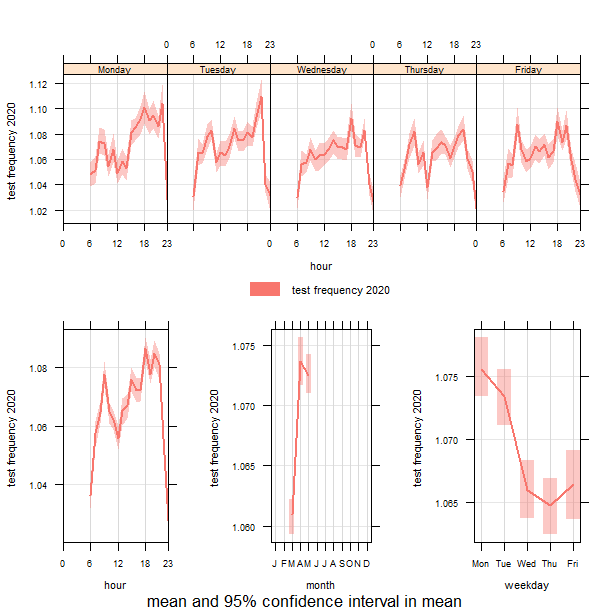
\includegraphics[width=0.85\textwidth,height=0.5\textheight]{figures/time.var.plot2020.png}
\caption{Speed tests over time, 2020 \label{test2020}}
\end{figure}

\begin{figure}
\centering
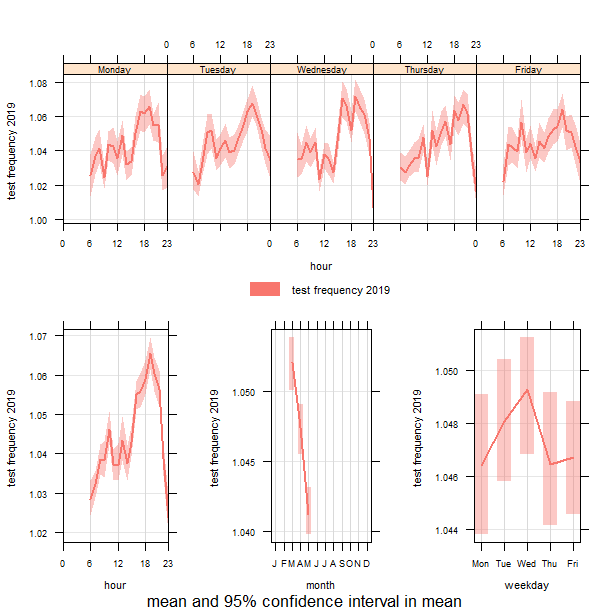
\includegraphics[width=0.85\textwidth,height=0.5\textheight]{figures/time.var.plot2019.png}
\caption{Speed tests over time, 2019 \label{test2019}}
\end{figure}

In Section \protect\hyperlink{sec:4.1}{4.1}, we review the temporal
profile of upload speed by hour of the day and day of the composite week
for each of the clusters. Since the quality and reliability of internet
services vary in time and space due to both supply and demand-side
influences, we also use a number of different measures to describe
experienced upload speeds per cluster. These include: i) mean,
experienced connection speed, ii) standard deviation or the amount of
fluctuation from the mean, and iii) the variation in speeds during the
new morning peak of testing when working from home is more likely to
take place. We take account of all three measurements in order to
determine how resilient broadband speeds are as experienced in different
parts of the UK during a time of extreme demand.

The cause of these different experiences of broadband resilience may
vary between and within clusters, as they may reflect either patterns of
demand or quality of infrastructure. Our approach is also limited by
potential endogeneity, as for example, better quality connections with
high mean speeds may enable more working from home, but greater demand
can cause slower speeds, less reliability, or greater variability of
speed at different times of day or week. Therefore, we avoid attributing
any cause to our analysis of the experienced level of quality and
reliability of upload speeds. Instead, we run an auxiliary regression to
understand how the spatial and temporal patterns of internet service
relate to the economic geography of the UK. More specifically, we
estimate the following multinomial logit model:

\begin{align}
Pr(Y_{i}=j) = \frac{exp^{X_{i}\beta_{j}}}{\sum_{i=1}^j exp^{X_{i}\beta_{j}}}
\begin{cases}
    i = 1, 2, ... , N \\  
    j = 1, 2, ... , J
\end{cases}\label{eq1}
\end{align}

Based on the outcomes of the time-series clustering, we identify \(J\)
distinct and crisp clusters. We then regress this cluster membership
against a vector \(X_{i}\) of socio-economic and geographic variables,
which are discussed in detail in the relevant Section
\protect\hyperlink{sec:4.2}{4.2}. Because we cannot identify individuals
or households and consequently aggregated our data at the LAD level, our
results offer correlations between the socioeconomic characteristics of
certain geographic locations and internet service quality, not a record
of who was telecommuting. Such individual data could be found though
surveys, but these offer less detailed information about the experience
of internet resilience due to enforced demand, which is the main
contribution of this paper. Our auxiliary regression, therefore,
provides an indication of how internet connectivity can reinforce or
redress existing spatial and social inequalities in different places.
However, it opens a path to future research by highlighting the
importance of understanding of how telecommuting capabilities and
digital infrastructure divisions intersect.

\hypertarget{sec:4}{%
\section{Results}\label{sec:4}}

\hypertarget{sec:4.1}{%
\subsection{Upload Clusters / cluster description}\label{sec:4.1}}

The temporal profiles of the local authority clusters have been
summarised in Figure \ref{UpCluster} and Table \ref{up.cluster.descr},
to provide an overview of the quality and reliability of experienced
broadband in different parts of the UK. Figure \ref{UpCluster} shows a
composite profile of mean upload speeds per hour per day for each of the
largest six clusters, in terms of the LAD membership and population.

\begin{figure}
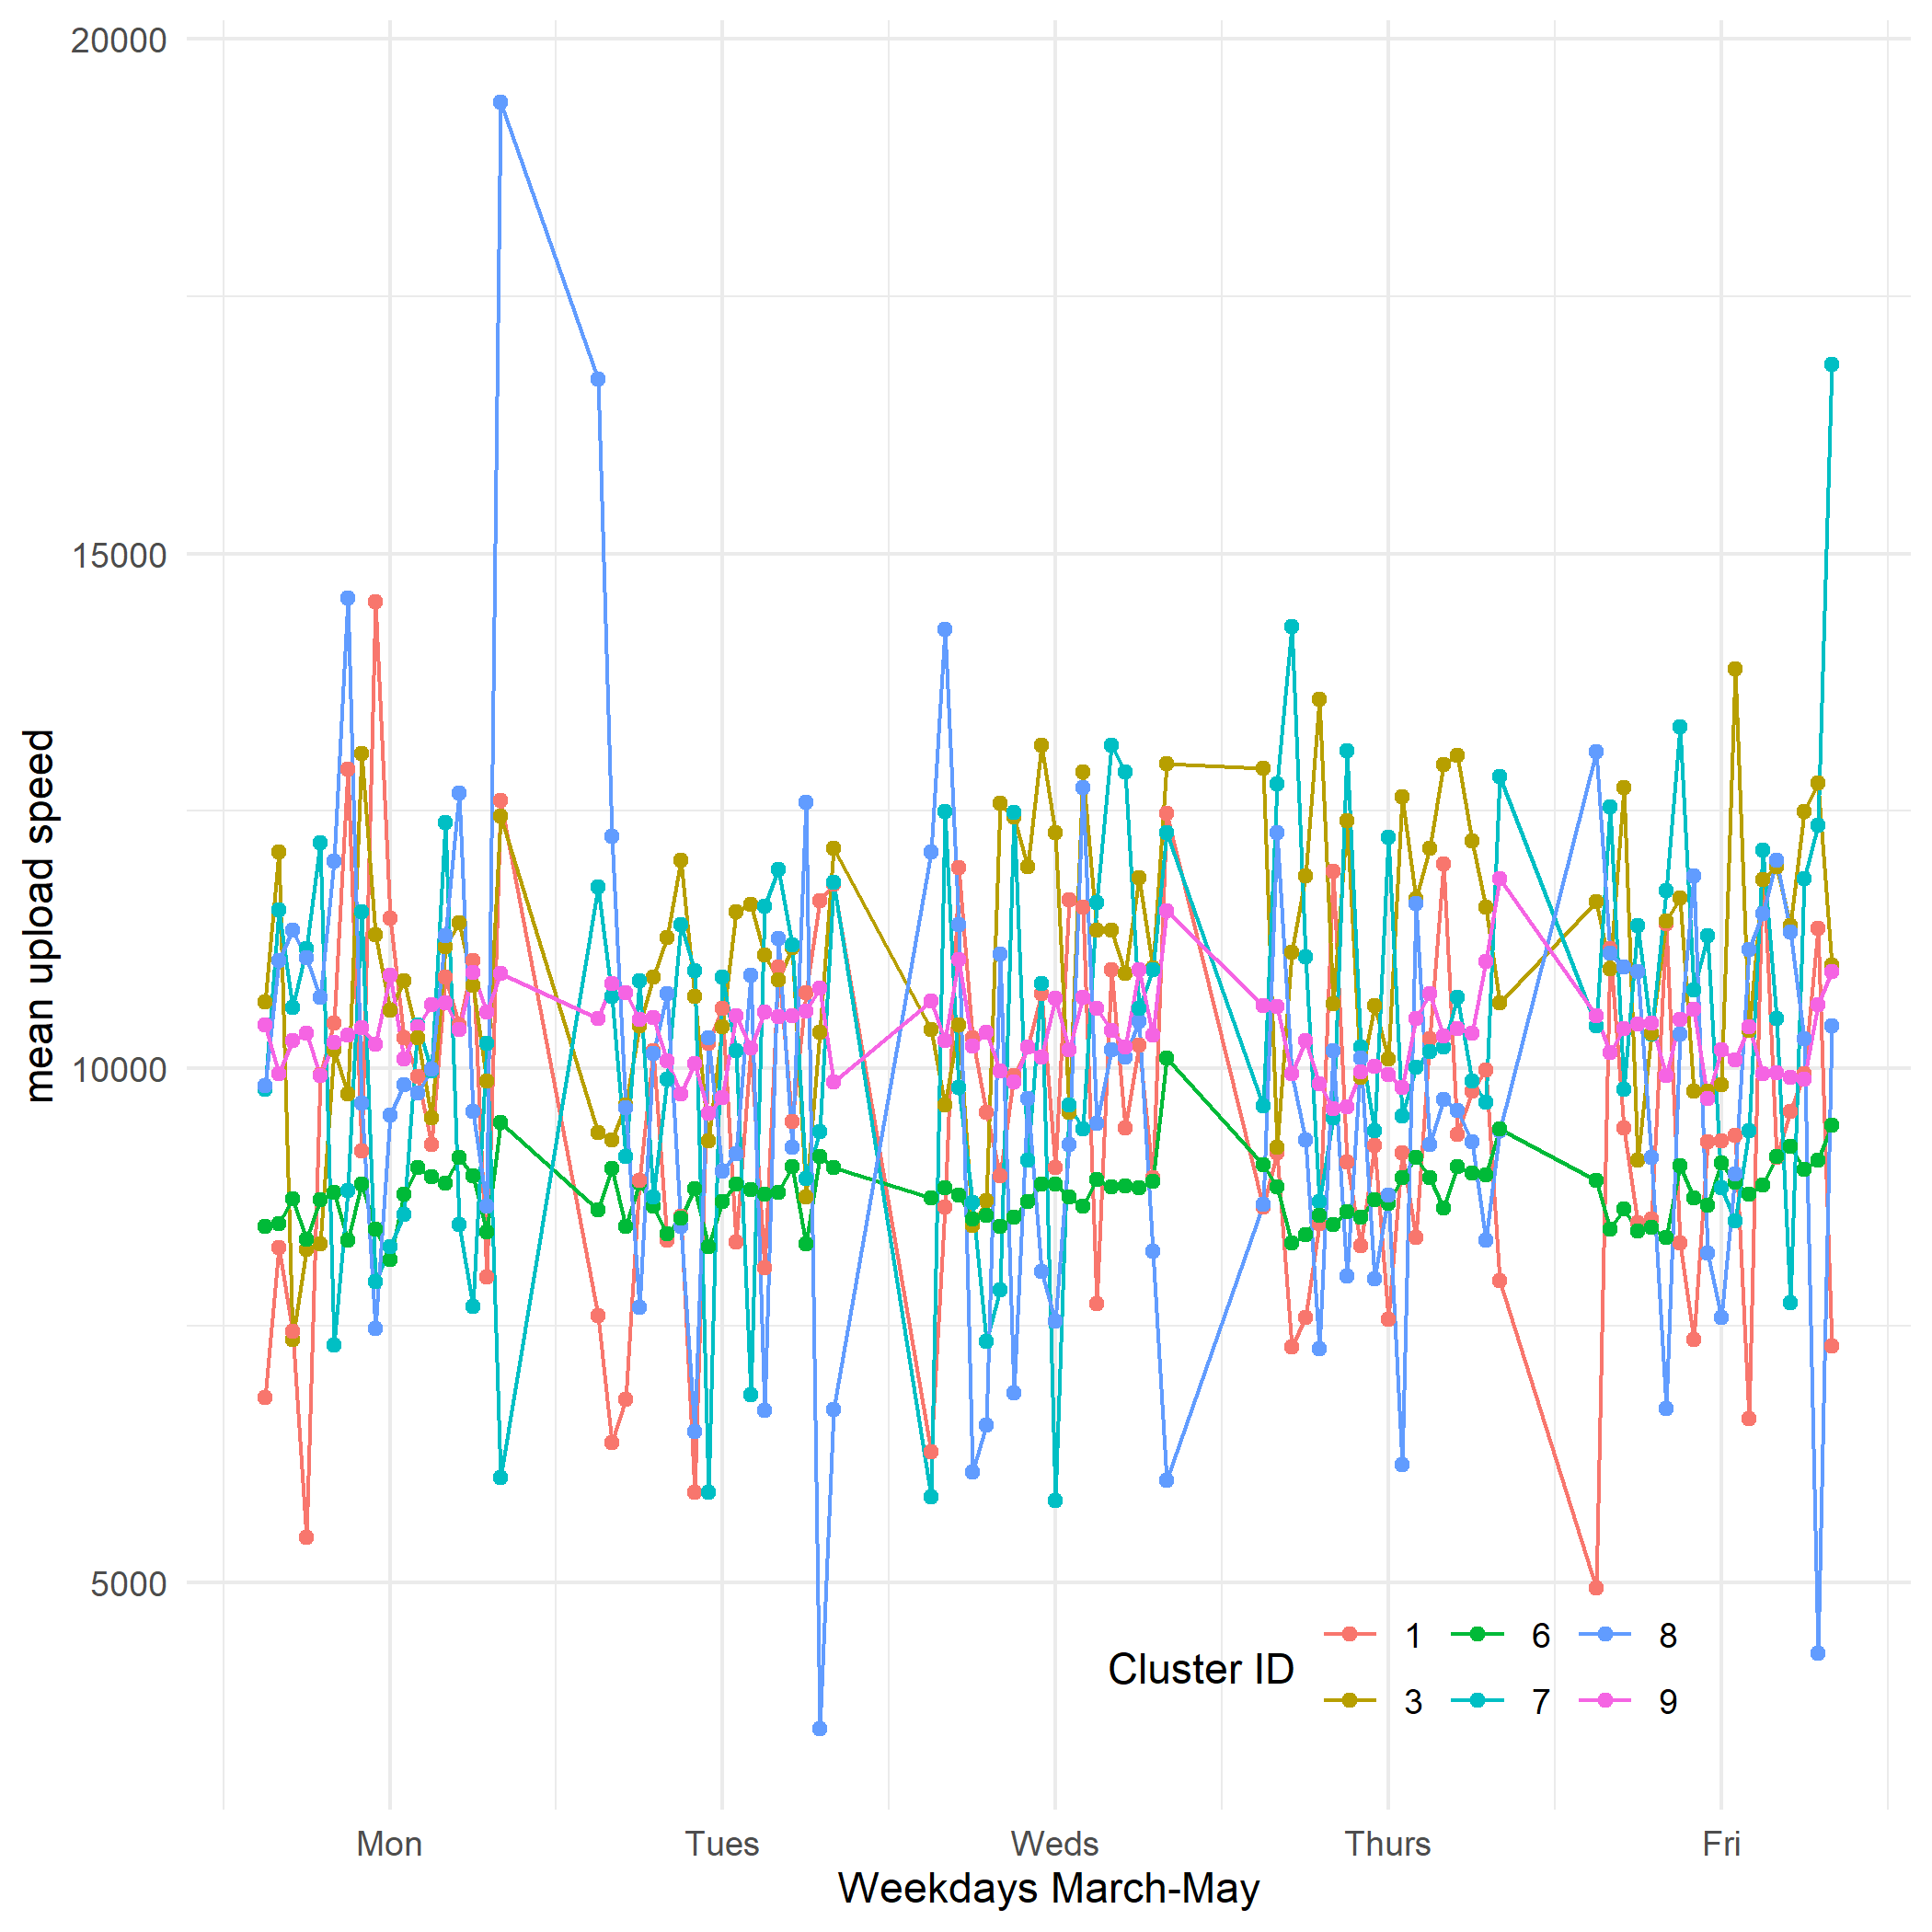
\includegraphics[width=0.95\linewidth]{figures/UpCluster} \caption{\label{UpCluster}Temporal profilies for upload speed clusters}\label{fig:unnamed-chunk-2}
\end{figure}

\begin{table}[!htbp] \centering 
  \caption{Upload speed cluster characteristics\label{up.cluster.descr}} 
  \label{} 
\footnotesize 
\begin{tabular}{@{\extracolsep{0pt}} ccccccc} 
\\[-1.8ex]\hline 
\hline \\[-1.8ex] 
Cluster & N. of LADs & LAD population & mean speed & SD speed & mean AM speed & mean PM speed \\ 
\hline \\[-1.8ex] 
1 & 9 & 903200 & 9564 & 6314 & 8798 & 10457 \\ 
2 & 2 & 162000 & 12085 & 6537 & 11882 & 10866 \\ 
3 & 12 & 1785800 & 11047 & 6079 & 10029 & 11634 \\ 
4 & 1 & 91100 & 9689 & 6122 & 7816 & 9689 \\ 
5 & 3 & 280000 & 10802 & 6116 & 11010 & 10084 \\ 
6 & 229 & 40552800 & 8761 & 5847 & 8555 & 8955 \\ 
7 & 5 & 682500 & 10326 & 6102 & 10045 & 11149 \\ 
8 & 6 & 510000 & 9769 & 6352 & 8989 & 10836 \\ 
9 & 115 & 21467800 & 10328 & 5915 & 10283 & 10333 \\ 
\hline \\[-1.8ex] 
\multicolumn{7}{l}{Note: All speed measures are upload speeds} \\ 
\end{tabular} 
\end{table}

The largest cluster, comprising \(229\) local authorities and over
\(40\) million people, is cluster \(6\), which has the slowest aggregate
mean upload speed of any cluster, and the highest ratio of the standard
deviation to the mean. This suggests that those living in local
authorities in this cluster experienced some of the lowest quality
broadband services in terms of upload speeds and reliability in the UK.
However, as shown in Figure \ref{map.up.clusters}, some of the most
rural areas of the UK are included in this cluster. If these areas
suffer most from first level digital divides as described in the
literature review, the low speeds in rural areas might be pulling down
the averages in other areas in this largest cluster. Also, since the
areas are clustered by their temporal profile across the working week,
the graph in Figure \ref{UpCluster} indicates that speeds in cluster
\(6\) are some of the more reliable. Table \ref{up.cluster.descr}
confirms that upload speeds in cluster \(6\) during the morning peak
from \(9:00\)-\(10:59\) were, on average, only \(4.5\)\% slower than in
the evening peak period between \(19:00\) and \(20:59\), when
entertainment purposes are likely to be using the most bandwidth.

\begin{figure}
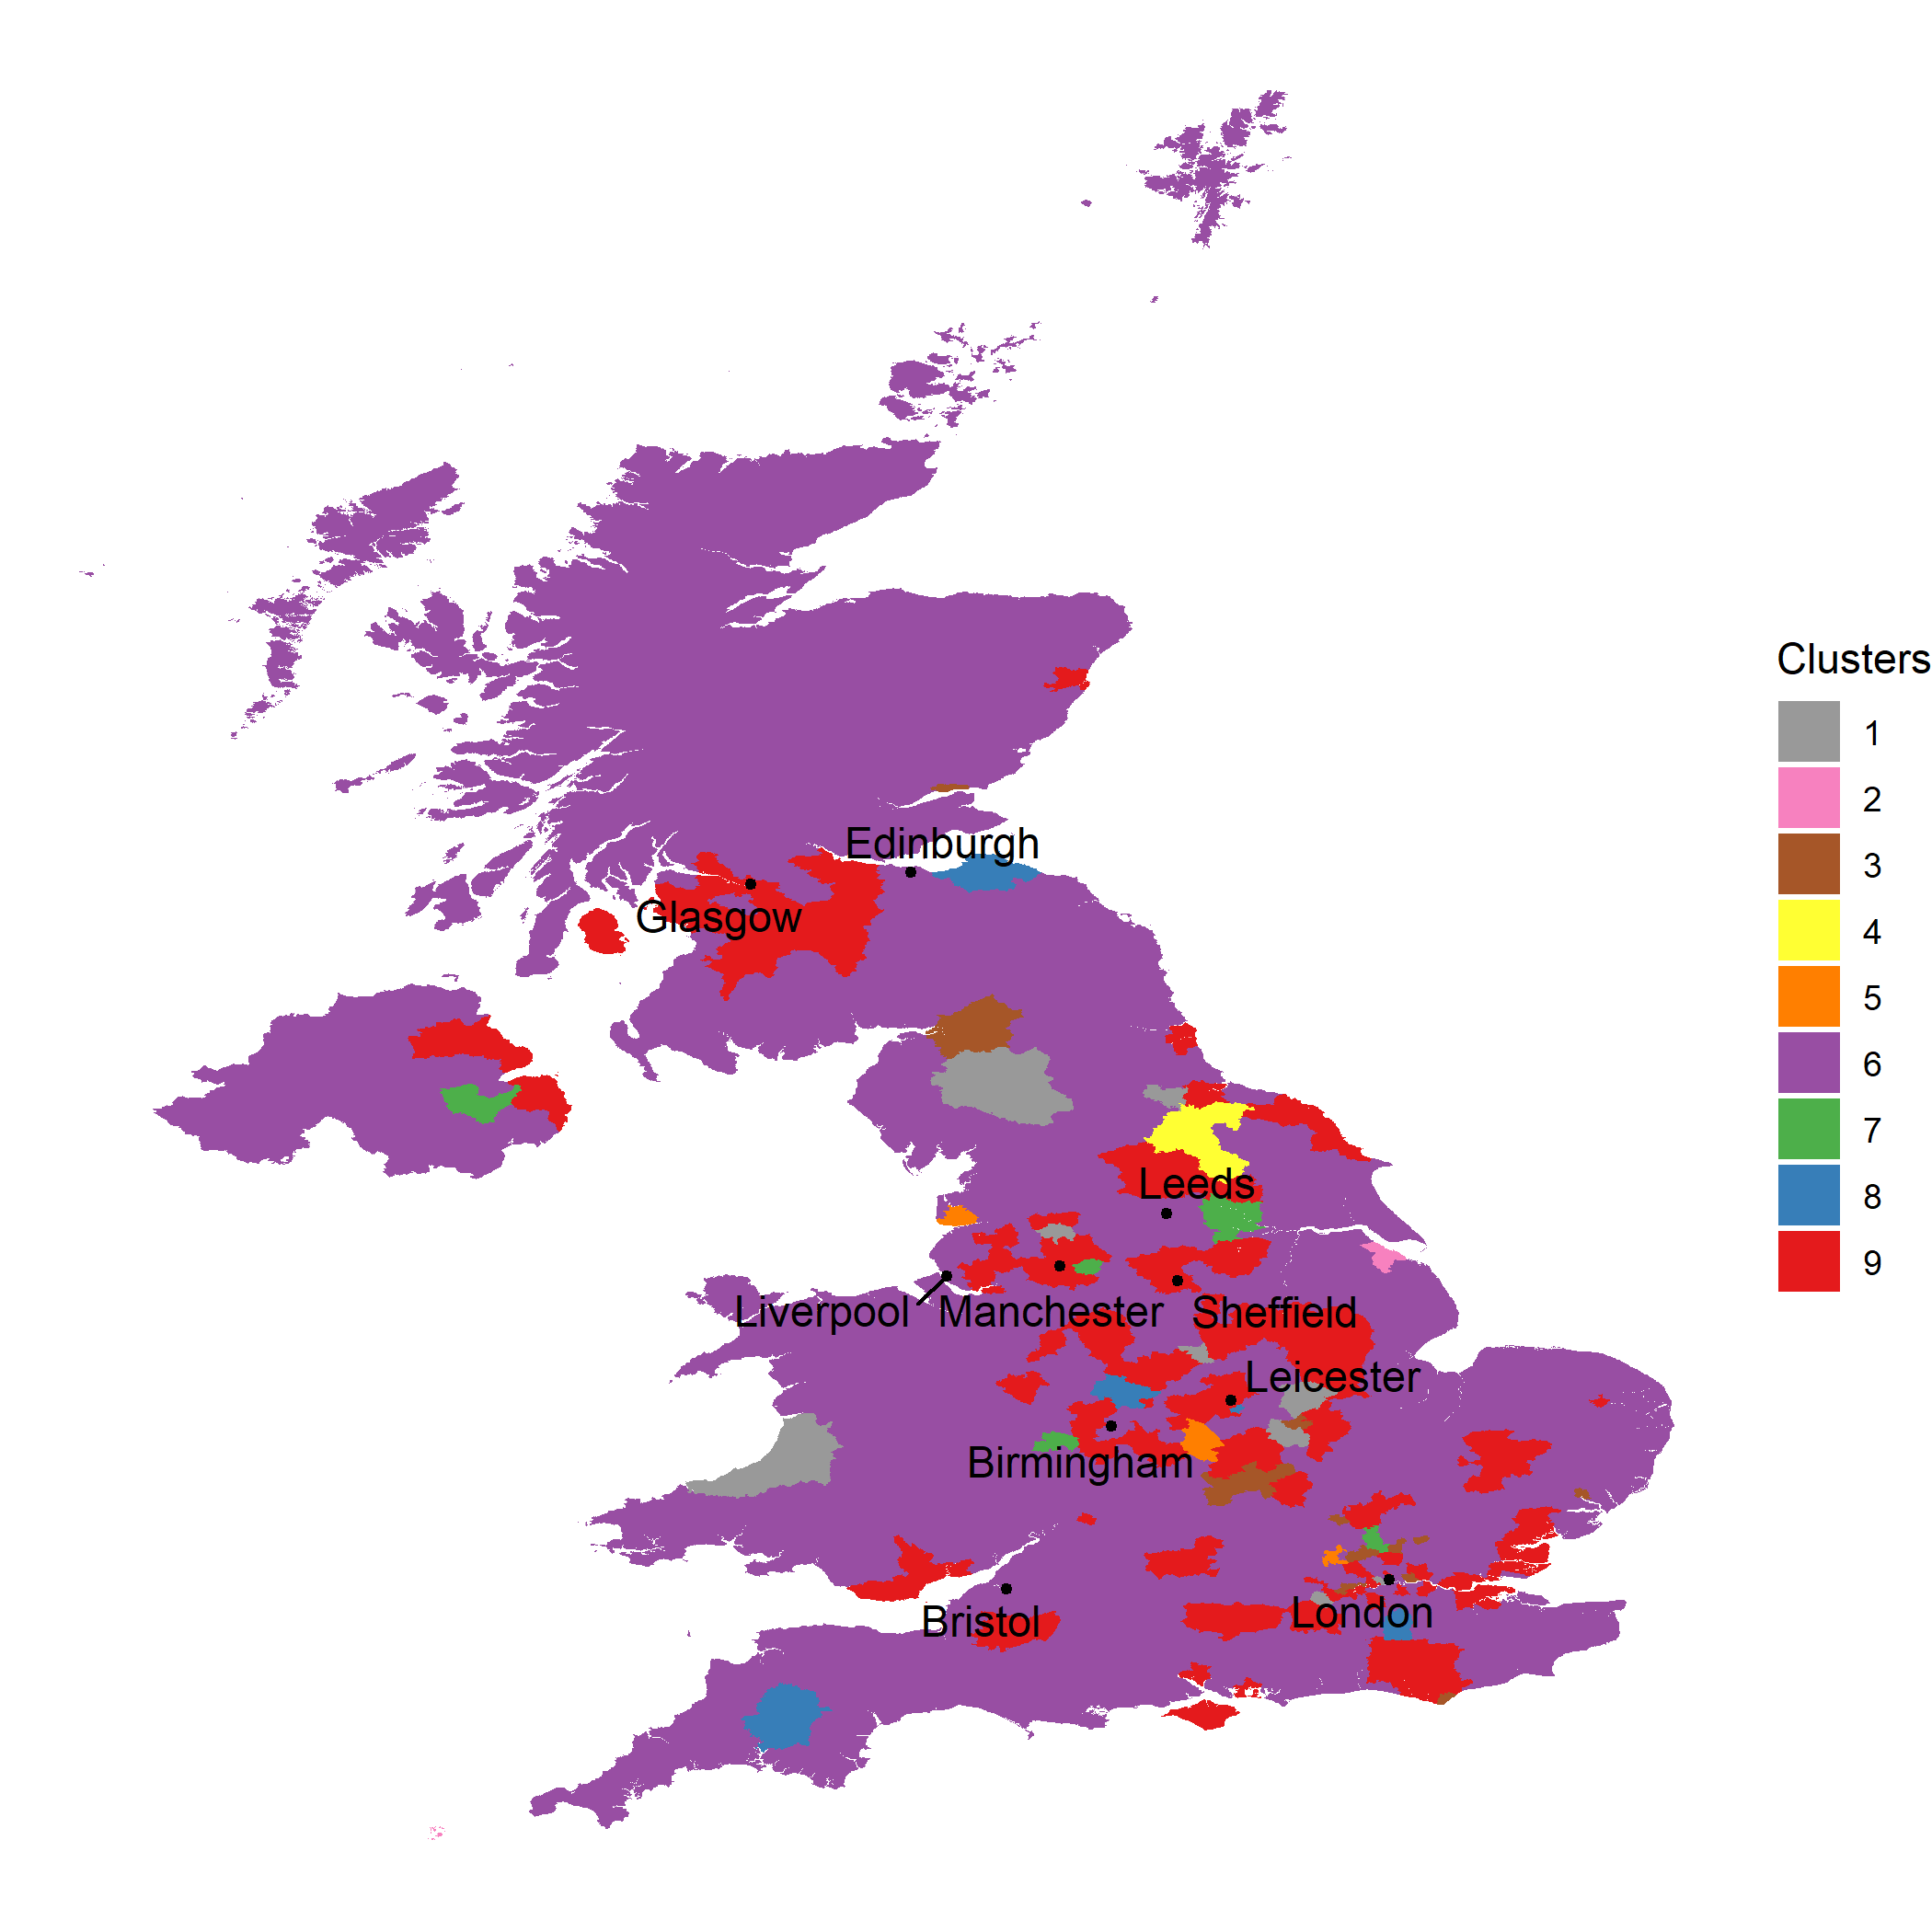
\includegraphics[width=0.95\linewidth]{figures/map.up.clusters} \caption{\label{map.up.clusters}Upload speed clusters for LADs}\label{fig:unnamed-chunk-4}
\end{figure}

Those living in the second largest cluster -- \(9\), with \(115\) LADs
and \(21.5\) million people -- experienced aggregate mean upload speeds
of more than \(1.5\)Mb/s faster than those in cluster \(6\), a lower
ratio of standard deviation to mean, and almost the same upload speeds
in the AM Peak as the PM Peak. Indeed, the temporal profile for cluster
\(9\) in Figure \ref{UpCluster}, like that for cluster \(6\), is fairly
flat. Whilst it is likely that the large numbers of tests being
performed by the large populations in these two clusters of LADs result
in less varied averages to show in the graph, the method of shape-based
clustering suggests that these results indicate that the majority of the
population of the UK experience less temporal variation, and so belong
in these two clusters. The results also confirm that those in cluster
\(9\) experienced a consistently better service during lockdown than
those in cluster \(6\), in terms of both average speed and reliability.

Of the smaller clusters, the \(15\) LADs in clusters \(1\) and \(8\),
home to over \(1.4\) million people, not only experience fairly average
upload speeds and high ratios of standard deviation to the mean, but
also experience much lower speeds during the morning peak than the
evening peak. From the large spikes and dips shown on Figure
\ref{UpCluster}, it is likely that this poor reliability or consistency
of morning internet speeds was more noticeable to those in cluster
\(1\), whilst those in cluster \(8\) experienced the lack of reliable
service as a problem throughout the day. Meanwhile, cluster \(7\)
experiences quite similar mean speeds to cluster \(9\), and a not too
dissimilar standard deviation, but mean speeds in the morning peak are
almost \(10\)\% lower than the evening peak. Cluster \(3\) boasts speeds
almost \(1\)Mb/s higher again, but suffers from even greater slowdown in
the morning peak. In comparison, clusters \(2\) and \(5\), home to a
little less than half a million people, experience not only above
average mean speeds, but also faster speeds in the morning peak compared
to the evening. Thus, in the five LADs in these two clusters, the
temporal profile of internet use may be closer to what might have been
expected pre-pandemic.

It is worth noting here that when we apply the same methods to upload
speed data for the same time period in 2019, the spatial distribution
and composition of the nine clusters of LADs are very different -- see
Appendix \protect\hyperlink{appendix2}{2}. This difference is an
indication of the changes in the temporal profile of internet usage that
took place during the pandemic, and which would be independent of any
wider trend in improving internet services.

In summary, the reliability of internet services during the working day
appears to have altered for the vast majority of locations due to
increased use from residents told to stay at home, and, if they were
fortunate, work from home. Yet this experience has been different in
different locations. In particular, LADs in cluster \(9\) experienced
higher speeds and more resilient broadband internet than those in the
largest cluster, \(6\). Those in clusters \(3\) and \(7\) also
experience higher mean speeds and better service reliability, and can be
more confident that they are on the right side of the first level
digital divide, and that their more resilient ICT infrastructure and
services can robustly support higher levels of telecommuting. On the
other hand, whilst high levels of telecommuting may be the cause of
morning speeds over 15\% lower than those in the evening, those in
clusters \(1\) and \(8\) also experience lower mean speeds than clusters
\(3\), \(7\), and \(9\), but not as low as cluster \(6\). Whilst the
differences may not be large, the lower upload speeds in cluster \(6\)
or the poor reliability in clusters \(1\) and \(8\) could still have had
implications for economic resilience if combined with other types of
digital divide. This potential will be explored in the next section.

\hypertarget{sec:4.2}{%
\subsection{Post-clustering regression analysis}\label{sec:4.2}}

\begin{sidewaystable}[!htbp] \centering 
  \caption{Auxiliary multinomial regression of upload speed clusters on socio-economic and geographic LAD variables\label{aux}} 
  \label{} 
\tiny 
\begin{tabular}{@{\extracolsep{5pt}}lcccccccc} 
\\[-1.8ex]\hline 
\hline \\[-1.8ex] 
\\[-1.8ex] & 1 & 2 & 3 & 5 & 6 & 7 & 8 & 9 \\ 
\\[-1.8ex] & (1) & (2) & (3) & (4) & (5) & (6) & (7) & (8)\\ 
\hline \\[-1.8ex] 
 pop, 2018 & $-$0.00004$^{**}$ & 0.00002 & 0.00001 & 0.00002 & 0.00001 & 0.00002 & $-$0.00000 & 0.00001 \\ 
  & (0.00002) & (0.00001) & (0.00001) & (0.00002) & (0.00001) & (0.00001) & (0.00002) & (0.00001) \\ 
  & & & & & & & & \\ 
 job density, 2018 & $-$0.534$^{***}$ & $-$0.362$^{***}$ & 4.211$^{***}$ & $-$0.890$^{***}$ & 3.516$^{***}$ & $-$8.624$^{***}$ & $-$3.259$^{***}$ & 3.337$^{***}$ \\ 
  & (0.00000) & (0.00000) & (0.00000) & (0.00000) & (0.00000) & (0.00000) & (0.00000) & (0.00000) \\ 
  & & & & & & & & \\ 
 distance to nearest met. area & $-$0.007$^{***}$ & 0.013$^{***}$ & 0.002$^{***}$ & 0.023$^{***}$ & $-$0.001 & $-$0.158$^{***}$ & 0.005$^{***}$ & $-$0.003$^{**}$ \\ 
  & (0.0004) & (0.00001) & (0.0003) & (0.0002) & (0.002) & (0.0001) & (0.0003) & (0.002) \\ 
  & & & & & & & & \\ 
 distance to London & 0.011$^{***}$ & 0.004$^{***}$ & 0.005$^{**}$ & $-$0.013$^{***}$ & 0.010$^{***}$ & 0.012$^{***}$ & 0.008$^{***}$ & 0.008$^{***}$ \\ 
  & (0.001) & (0.00004) & (0.002) & (0.001) & (0.001) & (0.001) & (0.002) & (0.001) \\ 
  & & & & & & & & \\ 
 South of the UK & $-$3.628$^{***}$ & 0.958$^{***}$ & 4.936$^{***}$ & $-$10.243$^{***}$ & 4.830$^{***}$ & 3.919$^{***}$ & $-$1.140$^{***}$ & 3.188$^{***}$ \\ 
  & (0.000) & (0.000) & (0.00000) & (0.00000) & (0.00001) & (0.00000) & (0.00000) & (0.00001) \\ 
  & & & & & & & & \\ 
 managerial jobs, 2020 & 0.944$^{***}$ & 0.628$^{***}$ & 0.593$^{***}$ & $-$0.544$^{***}$ & 0.634$^{***}$ & $-$0.128$^{***}$ & 0.725$^{***}$ & 0.511$^{***}$ \\ 
  & (0.00002) & (0.00000) & (0.00003) & (0.00003) & (0.00002) & (0.00003) & (0.00003) & (0.00002) \\ 
  & & & & & & & & \\ 
 tech jobs, 2020 & 0.350$^{***}$ & $-$0.222$^{***}$ & $-$0.068$^{***}$ & $-$0.151$^{***}$ & 0.018$^{***}$ & $-$0.139$^{***}$ & 0.143$^{***}$ & $-$0.071$^{***}$ \\ 
  & (0.00002) & (0.00000) & (0.00002) & (0.0001) & (0.00003) & (0.0001) & (0.00003) & (0.00003) \\ 
  & & & & & & & & \\ 
 skilled trade jobs, 2020 & 0.521$^{***}$ & 0.171$^{***}$ & 0.214$^{***}$ & $-$0.578$^{***}$ & 0.231$^{***}$ & 1.067$^{***}$ & 0.284$^{***}$ & 0.049$^{***}$ \\ 
  & (0.00002) & (0.00000) & (0.00004) & (0.00004) & (0.00004) & (0.0001) & (0.00003) & (0.00003) \\ 
  & & & & & & & & \\ 
 professional jobs, 2020 & $-$0.577$^{***}$ & $-$0.962$^{***}$ & $-$0.565$^{***}$ & $-$0.860$^{***}$ & $-$0.566$^{***}$ & $-$1.139$^{***}$ & $-$0.389$^{***}$ & $-$0.702$^{***}$ \\ 
  & (0.00003) & (0.00000) & (0.00004) & (0.0001) & (0.00004) & (0.0001) & (0.0001) & (0.00004) \\ 
  & & & & & & & & \\ 
 administrative jobs, 2020 & 0.200$^{***}$ & $-$1.324$^{***}$ & $-$0.050$^{***}$ & 0.136$^{***}$ & $-$0.137$^{***}$ & $-$0.101$^{***}$ & $-$0.018$^{***}$ & $-$0.155$^{***}$ \\ 
  & (0.00002) & (0.00000) & (0.00002) & (0.00004) & (0.00002) & (0.00005) & (0.00002) & (0.00002) \\ 
  & & & & & & & & \\ 
 service jobs, 2020 & $-$0.082$^{***}$ & $-$0.180$^{***}$ & $-$0.659$^{***}$ & $-$1.066$^{***}$ & $-$0.746$^{***}$ & $-$0.944$^{***}$ & $-$0.773$^{***}$ & $-$0.783$^{***}$ \\ 
  & (0.00002) & (0.00000) & (0.00003) & (0.00002) & (0.00002) & (0.00003) & (0.00002) & (0.00001) \\ 
  & & & & & & & & \\ 
 machine operation jobs, 2020 & 0.210$^{***}$ & 0.574$^{***}$ & 0.439$^{***}$ & $-$0.589$^{***}$ & 0.229$^{***}$ & $-$0.260$^{***}$ & 0.080$^{***}$ & 0.127$^{***}$ \\ 
  & (0.00001) & (0.00000) & (0.00002) & (0.00002) & (0.00001) & (0.00002) & (0.00001) & (0.00001) \\ 
  & & & & & & & & \\ 
 earnings, 2019 & $-$0.003$^{***}$ & 0.029$^{***}$ & 0.019$^{***}$ & 0.069$^{***}$ & 0.018$^{***}$ & 0.050$^{***}$ & 0.016$^{***}$ & 0.026$^{***}$ \\ 
  & (0.001) & (0.0001) & (0.001) & (0.002) & (0.001) & (0.002) & (0.001) & (0.001) \\ 
  & & & & & & & & \\ 
 n. business est. per hab., 2019 & 1.930$^{***}$ & $-$0.377$^{***}$ & 0.826$^{***}$ & 0.251$^{***}$ & 0.315$^{***}$ & 1.515$^{***}$ & $-$0.948$^{***}$ & $-$4.011$^{***}$ \\ 
  & (0.00000) & (0.000) & (0.00000) & (0.00000) & (0.00000) & (0.00000) & (0.00000) & (0.00000) \\ 
  & & & & & & & & \\ 
 furloughed per hab., 2020 & $-$1.518$^{***}$ & $-$0.152$^{***}$ & 11.014$^{***}$ & 0.972$^{***}$ & $-$26.969$^{***}$ & 2.059$^{***}$ & 4.236$^{***}$ & 10.500$^{***}$ \\ 
  & (0.00000) & (0.00000) & (0.00000) & (0.00000) & (0.00000) & (0.00000) & (0.00000) & (0.00000) \\ 
  & & & & & & & & \\ 
 AM tests per hab., 2020 & 0.002$^{***}$ & $-$0.011$^{***}$ & $-$0.140$^{***}$ & 0.015$^{***}$ & 0.231$^{***}$ & 0.005$^{***}$ & $-$0.025$^{***}$ & $-$0.078$^{***}$ \\ 
  & (0.000) & (0.000) & (0.000) & (0.000) & (0.000) & (0.000) & (0.000) & (0.000) \\ 
  & & & & & & & & \\ 
 Virgin Media \%, 2020 & $-$0.349$^{***}$ & 12.236$^{***}$ & 5.619$^{***}$ & 0.489$^{***}$ & 1.721$^{***}$ & $-$16.289$^{***}$ & $-$5.581$^{***}$ & 6.126$^{***}$ \\ 
  & (0.00000) & (0.00000) & (0.00000) & (0.00000) & (0.00000) & (0.00000) & (0.00000) & (0.00000) \\ 
  & & & & & & & & \\ 
 Constant & $-$4.570$^{***}$ & $-$1.045$^{***}$ & $-$6.539$^{***}$ & 5.629$^{***}$ & 2.957$^{***}$ & 3.386$^{***}$ & $-$2.531$^{***}$ & 2.979$^{***}$ \\ 
  & (0.00000) & (0.00000) & (0.00000) & (0.00000) & (0.00000) & (0.00000) & (0.00000) & (0.00000) \\ 
  & & & & & & & & \\ 
\hline \\[-1.8ex] 
McFadden's R squared & 0.435 & 0.435 & 0.435 & 0.435 & 0.435 & 0.435 & 0.435 & 0.435 \\ 
N & 322 & 322 & 322 & 322 & 322 & 322 & 322 & 322 \\ 
Akaike Inf. Crit. & 742.901 & 742.901 & 742.901 & 742.901 & 742.901 & 742.901 & 742.901 & 742.901 \\ 
\hline 
\hline \\[-1.8ex] 
\textit{Note:}  & \multicolumn{8}{r}{$^{*}$p$<$0.1; $^{**}$p$<$0.05; $^{***}$p$<$0.01} \\ 
\end{tabular} 
\end{sidewaystable}

Using an auxiliary multinomial logit regression, we test whether the
clusters that have higher mean speeds and more reliable services do
indeed consist of LADs that are more urban or closer to major urban
areas and are more likely to benefit from a choice of high quality
internet services. This part of the regression aims to confirm any first
level digital divides. Next, to better understand how the clusters fare
in relation to the second level digital divide, we consider which LADs
in which clusters have a higher proportion of occupations where the
nature of the work and the skills that occupation employs enable
telecommuting. Finally, we consider the rate of return on internet use,
or third level digital divides, by reviewing which clusters have the
highest earnings and job density, and also which clusters experienced
the highest share of population furloughed during this period in the
pandemic.

The results of the auxiliary regression are presented in Table
\ref{aux}. The dependent variable is the LAD cluster membership as
described in the \protect\hyperlink{sec:3}{methods and data} section and
equation \ref{eq1}. Each column represents a different cluster. The
reference case is cluster \(4\), which includes only the local authority
of Hambleton in North Yorkshire, a rural area of just over ninety
thousand people. Mean, experienced upload speed in cluster \(4\) (see
Table \ref{up.cluster.descr}) is close to the pre-clustered average for
the whole sample (\(9.3\)Mb/s). However, the standard deviation for
cluster \(4\) and the difference between average speeds in the morning
compared to the evening peak periods are indications of worse
reliability than many of the other clusters. Hence, the results in Table
\ref{aux} should be seen as relative rather than absolute probabilities.

First, we control for the number of speed tests run per cluster
inhabitant between \(9:00\)-\(10:59\) as well as the share of fast
Virgin Media internet connections \footnote{See Appendix
  \protect\hyperlink{appendix3}{3} for the descriptive statistics.}.
Regarding the former, we expect people in LADs with more unreliable
connections to test their internet speeds more often, and the results
show that those in cluster \(6\) are by far the most concerned about
reliability at that time of day. Meanwhile, those in clusters \(2\),
\(3\), and \(9\) benefit from a higher proportion of Virgin connections,
which is an indication that people in these clusters are more likely to
live in urban areas, with more profitable broadband markets, and a
better choice of broadband services. We also employ distance from London
and from the nearest metropolitan area (including London) as two
variables depicting peripherality and urban structure. However, whilst
significant, the pattern of coefficients of these variables is
inconclusive in confirmed first level digital divides. Even though
London was one of the ten largest metropolitan areas in England, which,
along with Glasgow and Cardiff, were identified to calculate the
variable estimating the impact of distance from the centre of a
metropolitan area, the coefficients for the two variables are mostly
small and the signs for some are opposite.

When looking at the constituent authorities (see full list of LADs in
Appendix \protect\hyperlink{appendix1}{1} as well as Figure
\ref{map.up.clusters}), however, Cluster \(9\) is clearly more urban,
including \(13\) of \(32\) London Boroughs, five of the seven
constitutent LADs of the West Midlands conurbation, nine of the ten
boroughs of Greater Manchester, and five of nine other large
metropolitan areas coded in for the `distance to nearest met area'
variable. Cluster \(9\) also includes the other main cities in the East
Midlands, Leicester and Derby, as well as smaller cities known for their
knowledge economy, such as Oxford and Milton Keynes. However, as
previously mentioned, there is more noise within the variables for the
two largest clusters than the smaller ones, and cluster \(6\) also
contains many urban areas. These include \(16\) London boroughs,
Birmingham City, Bolton in Greater Manchester, Leeds, Liverpool,
Newcastle and Bristol, as well as small cities with knowledge economies
such as Cambridge, Edinburgh, and Reading and its neighbours in the
high-tech agglomeration of the Thames Valley. And yet cluster \(6\) also
includes some of the most rural areas in the country, showing how
important it is to interpretation to consider the membership of the
cluster as well as the regression results.

The coefficients in Table \ref{aux} demonstrate that those in cluster
\(6\) were more likely to hold managerial, tech and professional jobs
than those in cluster \(9\), and were the least likely to be furloughed
of any cluster. Thus, although speeds were slow and not as reliable
during the morning peak as in cluster \(9\), the skills that enabled
telecommuting also enabled greater returns from doing so, despite lower
than average earnings. Cluster \(6\) also has the second highest job
density, with more jobs to keep. Likewise, those in LADs in clusters
\(1\) and \(8\) had the highest and second highest proportions of
residents working in tech or managerial occupations despite suffering
from lower speeds and unreliable services, another mismatch between
first and second level digital divides. Yet unlike cluster \(6\) and
despite occupations with better digital skills, cluster \(8\), with its
five peripheral suburban areas in the Midlands, Scotland and south of
London, as well as rural West Devon saw the third highest proportion of
its working population furloughed. It also had the second lowest average
earnings in 2019, suggesting that its population was more likely to be
on the wrong side of the third level digital divide before, as well as
during the pandemic. In contrast, the nine LADs of cluster \(1\), which
include more rural areas, plus Westminster in central London had the
lowest earnings of any cluster, but also lowest level of furlough after
cluster \(6\).

The regression results for cluster \(7\) also reveal the complexity of
intersecting and diverging digital divides. Along with \(3\) and \(9\),
the analysis in Section \protect\hyperlink{sec:4.1}{4.1} suggested this
cluster was on the `right' side of any first level digital divides, yet
the regression shows that it has the lowest proportion of Virgin
connections. It is furthest from a metropolitan area, but closest to
London. The five LADs in cluster \(7\) are all suburban, making it
sensible that the cluster is in the group with better infrastructure,
but none are central urban boroughs and, along with a London suburb,
Leeds suburb, Manchester suburb, and West Midlands suburb, the fifth LAD
is outside Belfast. Belfast was not included among the metropolitan
areas, and whilst there has been substantial investment in high speed
broadband in Northern Ireland in recent years, including by Virgin,
take-up may still lag behind historic networks in other urban markets.

Cluster \(7\) has the lowest proportion of residents currently employed
in professional occupations, and among the lowest proportions in
managerial or technical occupations. This suggests potentially a low
level of skills to take advantage of the quality internet service
available, a second level digital divide. Cluster \(7\) also has the
lowest job density. However, with the largest proportion of skilled
tradespeople, and the second highest number of businesses per
inhabitant, those in cluster \(7\) ranked second in terms of earnings in
2019. On the other hand, the lack of some of the occupations most likely
to telecommute during lockdown may have contributed both to a
substantial proportion being furloughed in 2020, and even to the
relative reliability of broadband speeds compared to many of the other
smaller clusters.

Cluster \(3\), meanwhile, had the greatest proportion of its workforce
furloughed of any cluster, despite having the highest job density and
the second highest average speeds. Ranking in the middle for most of the
occupations estimated, at least some of its population should have the
skills to work from home. The geography would suggest economic advantage
as well, with eight of its twelve LADs in the South of England,
including two London Boroughs, four suburban areas north of London, and
the two tightly bounded urban areas of Eastbourne and Ipswich -- a
greater proportion than any other cluster. Yet geographic position and
job density do not appear to equate to particularly high average
earnings in 2019, nor did they protect residents from furlough in 2020.
In contrast, cluster \(5\), comprised of three suburban districts in the
Northwest, Midlands, and the London green belt, had the highest average
earnings in 2019, despite low levels of residents working in managerial,
tech and professional occupations. Suburbs are considered the most
likely urban form in which telecommuters live \citep{e2018does}, yet the
contrast between these small, mainly suburban clusters -- \(7\), \(3\),
and \(5\), suggest that they are not all equally economically resilient
in a pandemic.

Cluster \(2\), which, like cluster \(5\), had faster morning broadband
speeds than evening speeds, as shown in Table \ref{up.cluster.descr}
contains two remote LADs, the Isles of Scilly and Northeast
Lincolnshire. Whilst the low demand may be due to the least residents in
tech occupations, it may also be due to high numbers of retired people.
Rural areas such as those in cluster \(2\) are often home to many older,
retired people \citep{blank2018local}, which may also explain some of
the contradictions in cluster \(1\) with its low levels of furlough and
low earnings, whilst the presence of Westminster in that cluster might
be why there are the highest levels of tech and managerial occupations.

In summary, the regression results indicate the complexity of measuring
second and third level digital divides within spatial aggregations where
the geography of first level digital divides has been captured using
time-series clustering of experienced broadband upload speeds as a
product of reliability not just availability. Whilst the differences in
mean speeds between clusters were not large, the temporal clustering of
internet resilience showed much greater variation, and was not spatially
dependent upon distance to large urban areas, or relative location.
Internet resilience supports a wide range of small and large urban
economies, but also fails, or at least frustrates a wide range of other
urban economies, as demonstrated by the number of morning peak tests per
capita run in cluster \(6\). Yet our analysis of the likelihood of
furlough within the population, especially in the smaller suburban
clusters \(7\), \(3\), \(5\), and \(8\) shows that digital divides were
as likely to diverge as intersect during the pandemic, and did not
necessarily overlap with prior economic divides. With a much greater
share of the population likely to continue to work from home in the
future, and with changing attitudes towards residential locations, our
analysis suggests that first level digital divides should be seen as a
function of reliability as well as availability, of upload speeds as
well as download speeds, and of greater spatial variation than might
have previously been considered.

\hypertarget{sec:5}{%
\section{Discussion and Conclusions}\label{sec:5}}

Our analysis demonstrated that the temporal profiles of seven of our
nine clusters had slower upload speeds in the morning than in the
evening. The opposite is likely to have been the norm prior to the
pandemic, as level of demand and bandwidth management is the most common
cause of temporal variation in experienced speeds, and why evening
download speeds, rather than daytime upload speeds, have been used to
benchmark the performance of internet services. Thus, the new patterns
can be taken as evidence of widespread telecommuting and other daytime
internet use which changed the temporal profile of internet activity
throughout the UK, not just in areas with more digital industry or
better skills. Furthermore, upload speeds have not previously been seen
as integral to universal service, considering there has never before
been such extreme demand for telecommuting and operations such as video
calls. Yet those in the largest cluster, \(6\), clearly experienced
lower upload speeds. Their speeds were also less reliable, perhaps
because they had higher levels of demand than the second largest
cluster, \(9\), where many more employees were furloughed. Indeed, those
with the skills and jobs to work from home were often left with the
least robust services and greatest slowdown.

Therefore, home-based digital infrastructure which considers upload
speeds and working day reliability as well as availability are likely to
be particularly important in a future where telecommuting might be a
more common means of accessing work and broadband services must be fit
for purpose. Although the long-term effects of such drastic changes in
telecommuting and attitudes towards working from home are difficult to
predict, the reliability of home broadband services deserve more
consideration than in the past. This would represent a switch from
previous demand-side broadband policies in the UK which tended to be
aimed at supporting small and medium enterprises
\citep{HENDERSON2020102024}. Such policies were based on previous
research regarding the productivity effects of broadband infrastructure
\citep{DESTEFANO2018110}. However, this stream of research tended not to
consider residential locations as places that host economic activity.
Such policies also made some assumptions about the quality of service in
residential markets that could be assured without government
intervention -- an assumption which our analysis suggest is not entirely
accurate.

Policy and development proposals should also consider how the potential
changes wrought by the pandemic span various aspects of economy and
society. Changes to transportation planning due to altered commuting
patterns also imply changes in land use and urban planning to
accommodate people who work from home
\citep{BUDNITZ2020102713, ELLDER2020102777}. Productivity and innovation
changes will reflect upon changes in agglomeration externalities and the
attraction of large cities \citep{econobs}. Further research may be able
to measure the economic resilience of the different clusters of places
discussed in this paper once this pandemic is firmly past. However, our
analysis demonstrates that the economic resilience made possible by
working from home cannot be understood without considering the
underpinning digital divides and cannot be achieved without planning for
how the levels of digital, social and economic divides might intersect.
For example, our results suggest that broadband policies cannot improve
the economic resilience of places where the industrial structure does
not align with occupations that incorporate the digital skills and
capabilities to work from home. Such places instead experienced higher
proportions of their labour force being placed on furlough.

Early research on Covid-19 and cities also speculated upon the changes
that potential extensive post-Covid working from home patterns might
generate for spatial structure: from more walkable cities and more
localised production and consumption patterns to more extensive urban
sprawl, the decline in public transportation and increased private car
usage \citep{batty2020editorial}. Despite the essential role it played
during the pandemic, less effort has been spent in understanding the
current and future role of digital infrastructure. Our results indicate
that probably for the first time the future of cities and spatial
structure are so intertwined with digital infrastructure. If the
post-covid world is a world with extensive working from home, then we
need to build, among other things, resilient digital infrastructure
capable of bridging the first layer of the digital divide. Contrary to
previous broadband business and deployment plans, emphasis should be
placed not only on download, but also on upload speeds
\citep{brake2020lessons}. In essence, Covid-19 accentuated the old
argument, now more valid than ever: digital infrastructure, just like
any other network infrastructure, only becomes visible when it stops
working \citep{star1999, tranos2013geography}.

On the other hand, the nuanced picture we gained through our analysis of
the UK case study suggests that being on the right side of the second
level digital divide had a greater impact on economic resilience and
therefore the third level digital divide, than having quality internet
connectivity. Our regressions results for cluster \(1\) and \(6\) are a
demonstration of this. Our analysis shows both the intersections and
divergences of digital and economic division. Almost all of the largest
urban areas in the UK, as well as many smaller cities, were split
between the largest two clusters -- \(6\) and \(9\) -- and both contain
LADs that are centres of the knowledge economy, from Cambridge in the
former to Oxford in the latter, or have high concentrations of digital
businesses, like Reading in the former and Milton Keynes in the latter
\citep{technation2017}. Yet whilst LADs in cluster \(9\) were able to
benefit both from reliable internet connections and populations familiar
with working from home to capitalise on their digital infrastructure,
they appeared to have a lower rate of return in the pandemic, with far
greater numbers furloughed. Is this an indication of historic economic
division, as well as the third level digital divide, in cities in the
North and Midlands unable to capitalise on their digital infrastructure?
Meanwhile, did the greater presence in London and the South of LADs in
cluster \(6\), as well as the inclusion of many rural areas less
impacted by the pandemic help those in this cluster be more resilient
and gain greater returns, despite using less reliable internet services?
Further research would be necessary to prise apart the detail,
particularly in the largest clusters where averages are less distinct.

In conclusion, this paper offers a new perspective on telecommuting from
the viewpoint of the complex web of digital divides. We employ novel
data regarding experienced upload speeds and time-series clustering
methods, a family of unsupervised machine learning techniques which are
rarely utilised in geographical research. Fast, reliable internet
connections are necessary for the population to be able to work from
home. Although not every place hosts individuals in occupations which
allow for telecommuting nor with the necessary skills to effectively use
the internet to telecommute, this paper raises the issue that places may
depend upon good internet reliability as well as connectivity to achieve
economic resilience in a period like the current pandemic when internet
resilience is so vital.

\hypertarget{supplemental-material}{%
\section*{Supplemental Material}\label{supplemental-material}}
\addcontentsline{toc}{section}{Supplemental Material}

The LAD upload clusters as well as the mean AM and PM upload speeds are
presented in the Supplemental Material. Download the .html file and open
it using your internet browser. Hovering over the LAD polygons provides
the mean internet speeds.

\hypertarget{acknowledgement}{%
\section*{Acknowledgement}\label{acknowledgement}}
\addcontentsline{toc}{section}{Acknowledgement}

The authors would like to thank
\url{https://www.broadbandspeedchecker.co.uk/} for providing the main
data used for this paper.

\pagebreak

\hypertarget{appendix1}{%
\section*{Appendix 1}\label{appendix1}}
\addcontentsline{toc}{section}{Appendix 1}

This is the LAD cluster membership for the upload speed timeseries.

\textbf{Cluster 1: } Ceredigion, Darlington, Eden, Erewash, Kettering,
Rossendale, Runnymede, Rutland, Westminster

\textbf{Cluster 2: } Isles of Scilly, North East Lincolnshire

\textbf{Cluster 3: } Broxbourne, Carlisle, Corby, Dundee City,
Eastbourne, Harlow, Hertsmere, Hounslow, Ipswich, Luton, Newham, South
Northamptonshire

\textbf{Cluster 4: } Hambleton

\textbf{Cluster 5: } Fylde, Rugby, Three Rivers

\textbf{Cluster 6: } Aberdeenshire, Adur, Allerdale, Amber Valley,
Angus, Antrim and Newtownabbey, Argyll and Bute, Armagh City, Banbridge
and Craigavon, Arun, Ashford, Aylesbury Vale, Babergh, Barnet,
Barrow-in-Furness, Basildon, Bassetlaw, Bath and North East Somerset,
Bedford, Belfast, Birmingham, Blackburn with Darwen, Blackpool, Blaenau
Gwent, Bolton, Boston, Bournemouth, Christchurch and Poole, Bracknell
Forest, Bradford, Braintree, Breckland, Brentwood, Bridgend, Brighton
and Hove, Bristol, City of, Broadland, Bromley, Calderdale, Cambridge,
Camden, Canterbury, Carmarthenshire, Causeway Coast and Glens, Central
Bedfordshire, Chelmsford, Cherwell, Cheshire East, Cheshire West and
Chester, Chesterfield, Chichester, Chiltern, City of Edinburgh, City of
London, Clackmannanshire, Conwy, Copeland, Cornwall, Cotswold, County
Durham, Coventry, Craven, Croydon, Dacorum, Dartford, Denbighshire,
Derbyshire Dales, Derry City and Strabane, Dorset, Dover, Dumfries and
Galloway, Ealing, East Cambridgeshire, East Devon, East Dunbartonshire,
East Hampshire, East Hertfordshire, East Lindsey, East Renfrewshire,
East Riding of Yorkshire, East Suffolk, Elmbridge, Epping Forest, Epsom
and Ewell, Exeter, Fareham, Fenland, Fermanagh and Omagh, Fife,
Flintshire, Folkestone and Hythe, Forest of Dean, Gateshead, Gloucester,
Gosport, Great Yarmouth, Greenwich, Gwynedd, Hackney, Harborough,
Haringey, Hartlepool, Hastings, Havering, Herefordshire, County of, High
Peak, Highland, Hillingdon, Horsham, Huntingdonshire, Inverclyde, Isle
of Anglesey, King's Lynn and West Norfolk, Kingston upon Hull, City of,
Kingston upon Thames, Kirklees, Lambeth, Lancaster, Leeds, Lincoln,
Liverpool, Maidstone, Malvern Hills, Mansfield, Melton, Merthyr Tydfil,
Mid Devon, Mid Suffolk, Mid Ulster, Midlothian, Mole Valley,
Monmouthshire, Moray, Na h-Eileanan Siar, Neath Port Talbot, New Forest,
Newcastle upon Tyne, Newry, Mourne and Down, North Devon, North East
Derbyshire, North Lanarkshire, North Lincolnshire, North Norfolk, North
Somerset, North Tyneside, North Warwickshire, North West Leicestershire,
Northumberland, Orkney Islands, Pembrokeshire, Pendle, Perth and
Kinross, Peterborough, Plymouth, Powys, Preston, Reading, Redcar and
Cleveland, Reigate and Banstead, Rhondda Cynon Taf, Ribble Valley,
Richmondshire, Rother, Rotherham, Rushcliffe, Rushmoor, Ryedale,
Scottish Borders, Sedgemoor, Sefton, Sevenoaks, Shetland Islands,
Shropshire, Somerset West and Taunton, South Ayrshire, South Bucks,
South Cambridgeshire, South Gloucestershire, South Hams, South Holland,
South Lakeland, South Norfolk, South Oxfordshire, South Ribble, South
Somerset, South Staffordshire, Southend-on-Sea, Southwark, St Albans,
Stafford, Stirling, Stoke-on-Trent, Stratford-on-Avon, Stroud, Swale,
Swansea, Swindon, Teignbridge, Tendring, Test Valley, Tewkesbury,
Thanet, Tonbridge and Malling, Torbay, Torfaen, Torridge, Tower Hamlets,
Tunbridge Wells, Uttlesford, Wakefield, Waltham Forest, Wandsworth,
Warrington, Watford, Waverley, Wellingborough, West Berkshire, West
Lancashire, West Lindsey, West Oxfordshire, Wiltshire, Winchester,
Windsor and Maidenhead, Wirral, Wokingham, Worcester, Worthing, Wrexham,
Wychavon, Wycombe, Wyre

\textbf{Cluster 7: } Lisburn and Castlereagh, Selby, Tameside, Welwyn
Hatfield, Wyre Forest

\textbf{Cluster 8: } Cannock Chase, East Lothian, Lichfield, Oadby and
Wigston, Tandridge, West Devon

\textbf{Cluster 9: } Aberdeen City, Ards and North Down, Ashfield,
Barking and Dagenham, Barnsley, Basingstoke and Deane, Bexley, Blaby,
Bolsover, Brent, Bromsgrove, Broxtowe, Burnley, Bury, Caerphilly,
Cardiff, Castle Point, Charnwood, Cheltenham, Chorley, Colchester,
Crawley, Daventry, Derby, Doncaster, Dudley, East Ayrshire, East
Northamptonshire, East Staffordshire, Eastleigh, Enfield, Falkirk,
Gedling, Glasgow City, Gravesham, Guildford, Halton, Hammersmith and
Fulham, Harrogate, Harrow, Hart, Havant, Hinckley and Bosworth,
Hyndburn, Isle of Wight, Islington, Kensington and Chelsea, Knowsley,
Leicester, Lewes, Lewisham, Maldon, Manchester, Medway, Mendip, Merton,
Mid and East Antrim, Mid Sussex, Middlesbrough, Milton Keynes, Newark
and Sherwood, Newcastle-under-Lyme, Newport, North Ayrshire, North
Hertfordshire, North Kesteven, Northampton, Norwich, Nottingham,
Nuneaton and Bedworth, Oldham, Oxford, Portsmouth, Redbridge, Redditch,
Renfrewshire, Richmond upon Thames, Rochdale, Rochford, Salford,
Sandwell, Scarborough, Sheffield, Slough, Solihull, South Derbyshire,
South Kesteven, South Lanarkshire, South Tyneside, Southampton,
Spelthorne, St.~Helens, Staffordshire Moorlands, Stevenage, Stockport,
Stockton-on-Tees, Sunderland, Surrey Heath, Sutton, Tamworth, Telford
and Wrekin, Thurrock, Trafford, Vale of Glamorgan, Vale of White Horse,
Walsall, Warwick, Wealden, West Dunbartonshire, West Lothian, West
Suffolk, Wigan, Woking, Wolverhampton, York

\hypertarget{appendix2}{%
\section*{Appendix 2}\label{appendix2}}
\addcontentsline{toc}{section}{Appendix 2}

\begin{figure}
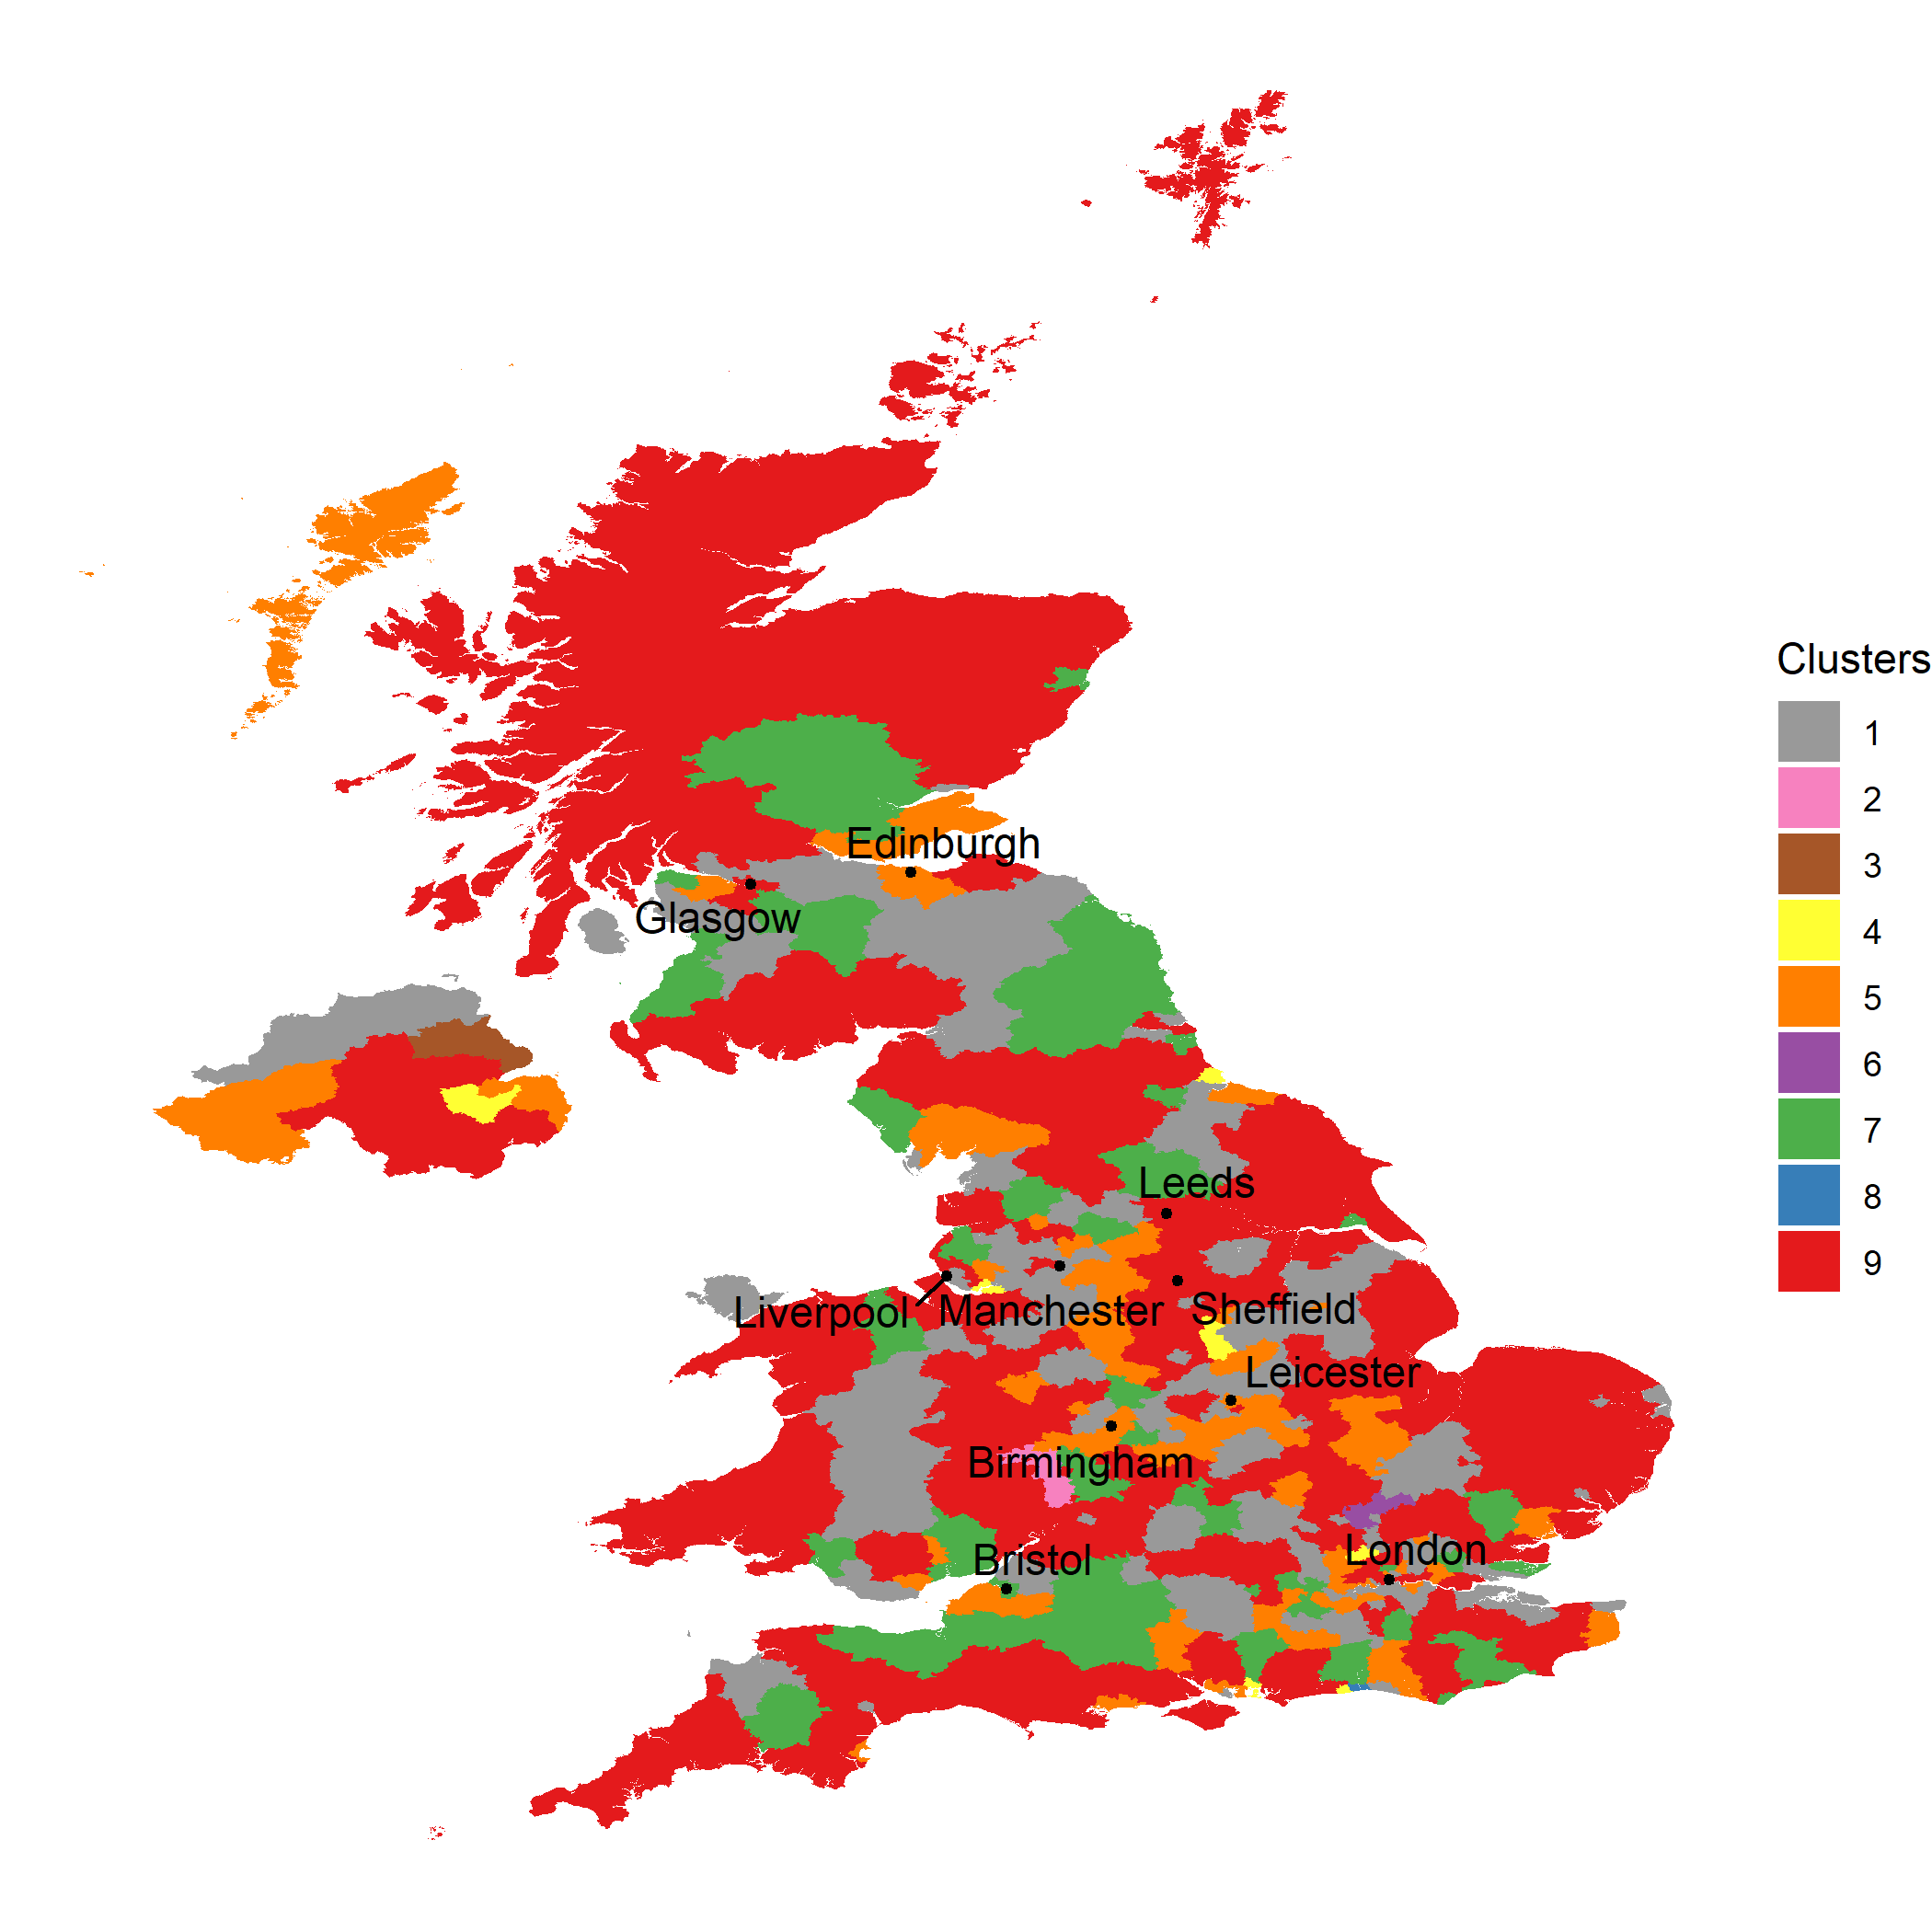
\includegraphics[width=1\linewidth]{figures/map.up.2019.clusters} \caption{\label{map.up.2019.clusters}Upload speed clusters for LADs in before the pandemic (2019)}\label{fig:unnamed-chunk-17}
\end{figure}

\pagebreak

\hypertarget{appendix3}{%
\section*{Appendix 3}\label{appendix3}}
\addcontentsline{toc}{section}{Appendix 3}

\begin{table}[!htbp] \centering 
  \caption{Descriptive statistics for the auxiliary regression explanatory variables\label{descr.aux}} 
  \label{} 
\footnotesize 
\begin{tabular}{@{\extracolsep{0pt}}lccccccc} 
\\[-1.8ex]\hline 
\hline \\[-1.8ex] 
Statistic & \multicolumn{1}{c}{N} & \multicolumn{1}{c}{Mean} & \multicolumn{1}{c}{St. Dev.} & \multicolumn{1}{c}{Min} & \multicolumn{1}{c}{Pctl(25)} & \multicolumn{1}{c}{Pctl(75)} & \multicolumn{1}{c}{Max} \\ 
\hline \\[-1.8ex] 
pop, 2018 & 365 & 174,952.100 & 119,557.100 & 8,700.000 & 100,400.000 & 214,900.000 & 1,141,400.000 \\ 
job density, 2018 & 365 & 1.137 & 5.726 & 0.400 & 0.700 & 0.930 & 110.110 \\ 
distance to nearest met. area & 365 & 53.269 & 57.700 & 0.150 & 22.050 & 69.290 & 544.090 \\ 
distance to London & 365 & 201.558 & 173.634 & 0.150 & 76.180 & 278.880 & 1,003.950 \\ 
south of the UK & 365 & 0.463 & 0.499 & 0.000 & 0.000 & 1.000 & 1.000 \\ 
managerial jobs, 2020 & 363 & 12.009 & 4.013 & 3.600 & 9.000 & 14.300 & 27.900 \\ 
tech jobs, 2020 & 364 & 14.505 & 4.057 & 3.500 & 11.800 & 16.900 & 29.600 \\ 
skilled trade jobs, 2020 & 358 & 10.513 & 3.764 & 1.000 & 8.025 & 12.500 & 21.600 \\ 
professional jobs, 2020 & 364 & 21.223 & 6.902 & 4.400 & 16.775 & 24.850 & 71.600 \\ 
administrative jobs, 2020 & 359 & 9.965 & 2.738 & 3.200 & 8.100 & 11.400 & 21.300 \\ 
service jobs, 2020 & 362 & 9.261 & 2.827 & 2.800 & 7.300 & 11.400 & 17.800 \\ 
machine operation jobs, 2020 & 337 & 6.339 & 2.847 & 1.200 & 4.400 & 7.900 & 19.800 \\ 
earnings, 2019 & 360 & 592.184 & 81.129 & 437.600 & 534.625 & 633.875 & 893.200 \\ 
Virgin Media \%, 2020 & 381 & 0.150 & 0.140 & 0.000 & 0.018 & 0.238 & 0.753 \\ 
n. business est. per hab., 2019 & 365 & 0.057 & 0.164 & 0.023 & 0.038 & 0.056 & 3.174 \\ 
AM tests per hab., 2020 & 365 & 0.0005 & 0.0002 & 0.0001 & 0.0003 & 0.001 & 0.001 \\ 
furloughed per hab., 2020 & 362 & 0.115 & 0.013 & 0.077 & 0.107 & 0.122 & 0.178 \\ 
\hline \\[-1.8ex] 
\end{tabular} 
\end{table}

\pagebreak

\bibliographystyle{tfcad}
\bibliography{bibliography.bib}




\end{document}
